\DeclareOption*{\PassOptionsToClass{\CurrentOption}{abntex2}}
\ProcessOptions

\documentclass[
	% -- opções da classe memoir --
	12pt,				% tamanho da fonte
	openright,			% capítulos começam em pág ímpar (insere página vazia caso preciso)
	oneside,			% para impressão em verso e anverso. Oposto a oneside
	a4paper,			% tamanho do papel. 
	% -- opções da classe abntex2 --
	%chapter=TITLE,		% títulos de capítulos convertidos em letras maiúsculas
	%section=TITLE,		% títulos de seções convertidos em letras maiúsculas
	%subsection=TITLE,	% títulos de subseções convertidos em letras maiúsculas
	%subsubsection=TITLE,% títulos de subsubseções convertidos em letras maiúsculas
	% -- opções do pacote babel --
	english,			% idioma adicional para hifenização
	french,				% idioma adicional para hifenização
	spanish,			% idioma adicional para hifenização
	brazil				% o último idioma é o principal do documento
	]{abntex2}

\usepackage{setspace}
\usepackage{conf-ifsc}	
\usepackage{hyperref}
\usepackage{graphicx}
\usepackage{caption}
\usepackage{subcaption}
\usepackage[utf8]{inputenc}
\usepackage{listings}
\usepackage{xcolor}
\usepackage{trivfloat}
\trivfloat{quadro}
\usepackage{enumitem}
\usepackage{xcolor}
\usepackage{multicol}
\usepackage{multirow}
\usepackage{hyperref}
\usepackage{float}
\floatstyle{plaintop}
\restylefloat{quadro}
\usepackage{chngcntr}
\usepackage{lipsum}
\usepackage{tocloft}
\usepackage{tocvsec2}
\usepackage{boxhandler}
\usepackage[font={bf,small},labelfont=small]{caption}
\usepackage{tikz}

\newcommand{\source}[1]{\caption*{\normalfont Fonte: {#1}}}


\counterwithout{equation}{chapter}
\counterwithout{figure}{chapter}
\counterwithout{table}{chapter}

\newcommand\ChangeRT[1]{\noalign{\hrule height #1}}


\definecolor{codegreen}{rgb}{0,0.6,0}
\definecolor{codegray}{rgb}{0.5,0.5,0.5}
\definecolor{codepurple}{rgb}{0.58,0,0.82}
\definecolor{backcolour}{rgb}{0.95,0.95,0.92}

\lstdefinestyle{mystyle}{
    backgroundcolor=\color{backcolour},   
    commentstyle=\color{codegreen},
    keywordstyle=\color{magenta},
    numberstyle=\tiny\color{codegray},
    stringstyle=\color{codepurple},
    basicstyle=\ttfamily\footnotesize,
    breakatwhitespace=false,         
    breaklines=true,                 
    captionpos=b,                    
    keepspaces=true,                 
    numbers=left,                    
    numbersep=5pt,                  
    showspaces=false,                
    showstringspaces=false,
    showtabs=false,                  
    tabsize=2
}

\lstset{style=mystyle}

%---------------------------------------------------------------------%
%---------------------------------------------------------------------%
% Informações de dados para CAPA e FOLHA DE ROSTO
%---------------------------------------------------------------------%
%---------------------------------------------------------------------%

\titulo{DESENVOLVIMENTO UMA BIBLIOTECA EM PYTHON PARA AUTOMATIZAR IDENTIFICAÇÃO E APROXIMAÇÃO DE GANHOS DE CONTROLADOR PARA SISTEMAS DE CONTROLE}

\autor{LUIZ FERNANDO NIQUELATTE}

\local{FLORIANÓPOLIS}

\data{2023.}

\orientador[Orientador:\\]{Prof. Cynthia Beatriz Scheffer Dutra, Prof.Dra.Eng.}


%\coorientador[Coorientador:\\]{Nome do coorientador}

\tipotrabalho{Monografia (Graduação)}

% O preambulo deve conter o tipo do trabalho, o objetivo, o nome da instituição e a área de concentração 
\preambulo{Trabalho de Conclusão de Curso submetido ao Instituto Federal de Educação, Ciência e Tecnologia de Santa Catarina como parte dos requisitos para obtenção do título de Engenheira Mecatrônica.}

% \textoaprovacao{Este Trabalho foi julgado adequado para obtenção do Título de Engenheira Eletrônica em abril de 2021 e aprovado na sua forma final pela banca examinadora do Curso de Engenharia Eletrônica do instituto Federal de Educação Ciência, e Tecnologia de Santa Catarina.}


%---------------------------------------------------------------------%
% Início do documento
%---------------------------------------------------------------------%

\begin{document}



\selectlanguage{brazil}
\frenchspacing 


% ----------------------------------------------------------
% ELEMENTOS PRÉ-TEXTUAIS
% ----------------------------------------------------------
% \pretextual

\imprimircapa
\imprimirfolhaderosto* %(o * indica que haverá a ficha bibliográfica)

%---------------------------------------------------------------------%
% ATENÇÃO - Pergunte para a Biblioteca do IFSC
% Inserir a ficha bibliografica - 
%
% Para gerar a ficha catalográfica acesse:
% http://ficha.florianopolis.ifsc.edu.br/
% Precisa ser feito pelo navegador Mozilla Firefox
%---------------------------------------------------------------------%

\imprimirficha{pdf/fichacatalografica.pdf}
%\cleardoublepage

%---------------------------------------------------------------------%
% Inserir folha de aprovação
%---------------------------------------------------------------------%


%\imprimiraprovacao
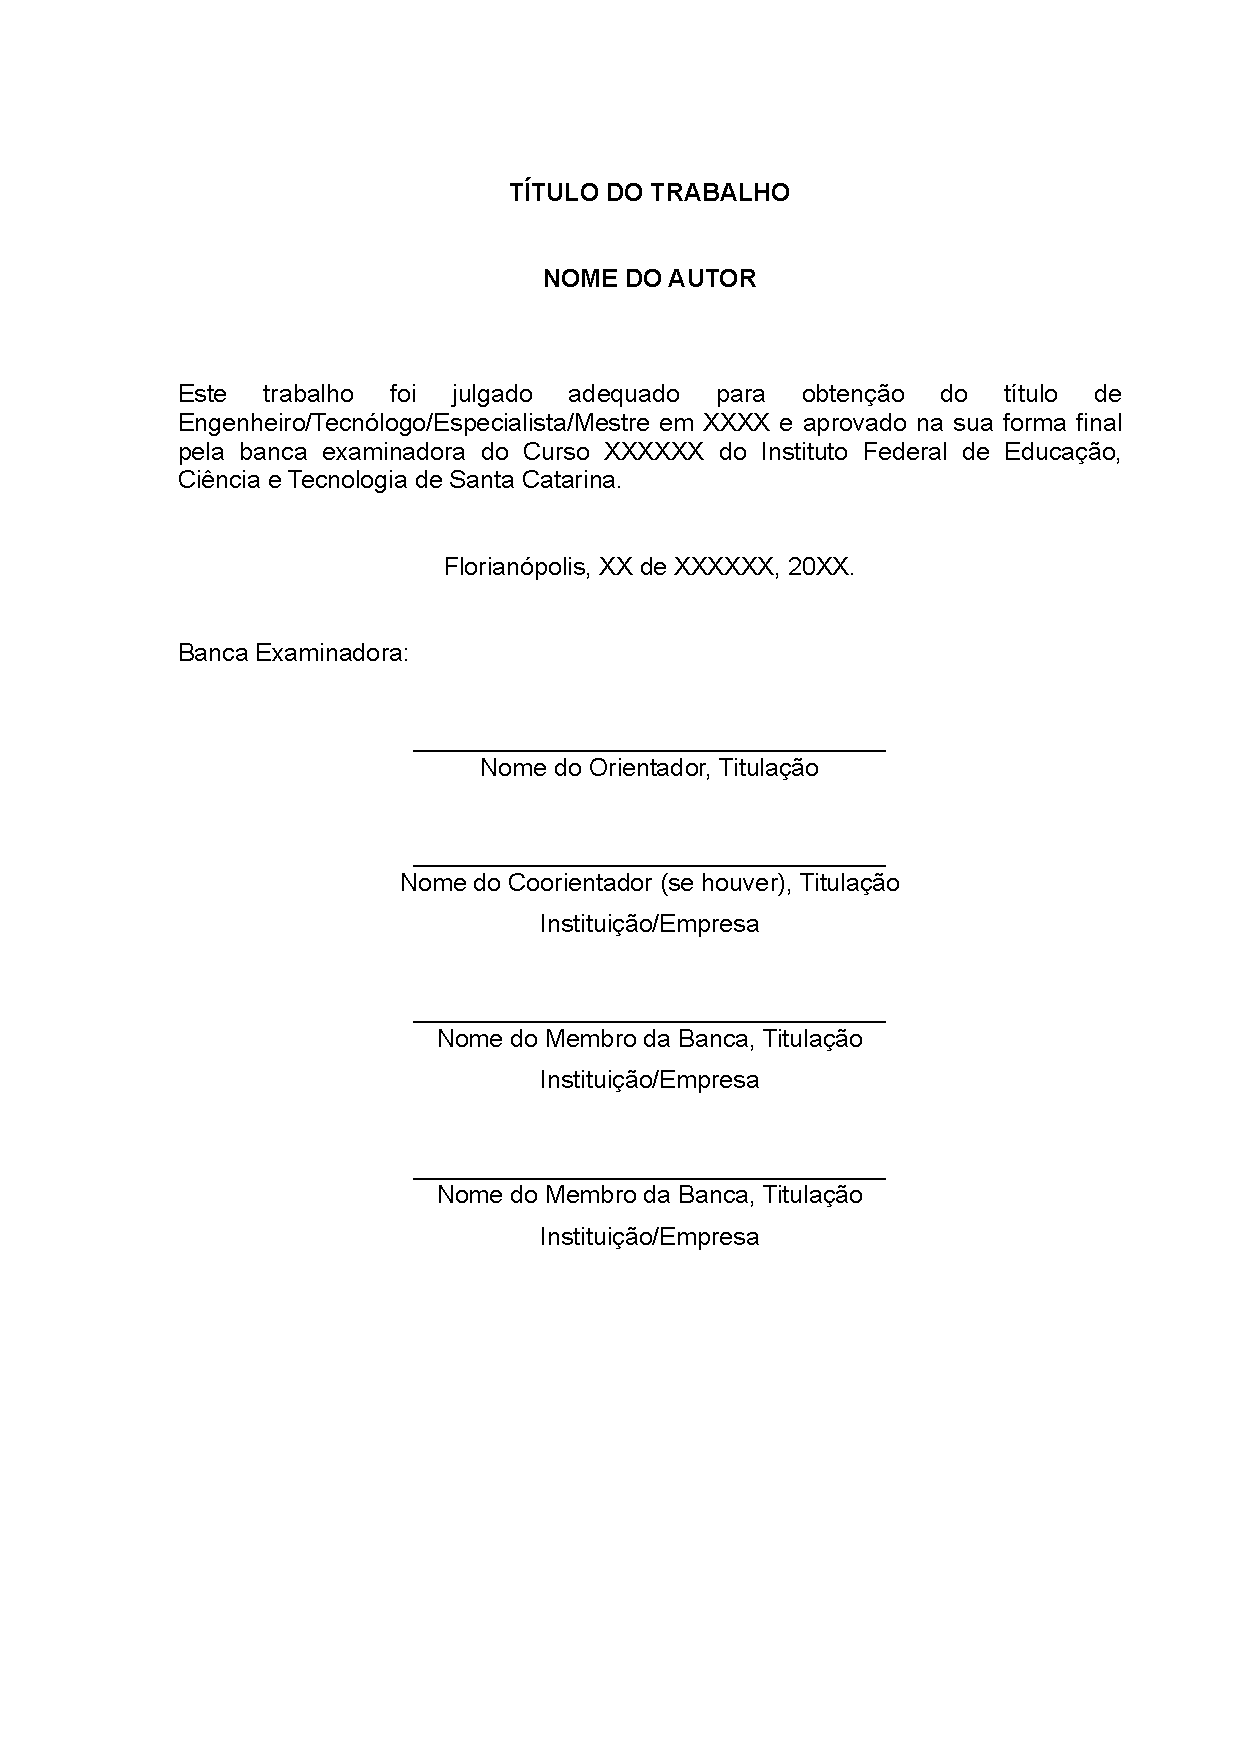
\includepdf[pages=-]{pdf/tcc-aprovado.pdf}

%\cleardoublepage

%---------------------------------------------------------------------%
% Dedicatória
%---------------------------------------------------------------------%
%\begin{dedicatoria}
%    \vspace*{\fill}
%	\begin{flushright}
%    		(Dedicatória é um elemento opcional.\\
%            Texto alinhado no canto inferior direito.\\
%            Não deve ultrapassar uma página.)
%	\end{flushright}
%\end{dedicatoria}




%---------------------------------------------------------------------%
% Agradecimentos
%---------------------------------------------------------------------%
\begin{agradecimentos}
    Elemento opcional que não pode ultrapassar o limite de uma página.
\end{agradecimentos}
% ---

%---------------------------------------------------------------------%
% Epígrafe
%---------------------------------------------------------------------%
%\begin{epigrafe}
%    \vspace*{\fill}
%	\begin{flushright}
%    		(Epígrafe é um elemento opcional.\\
%    		Texto alinhado no canto inferior direito.\\
%            Não deve ultrapassar uma página.)
%	\end{flushright}
%\end{epigrafe}

%---------------------------------------------------------------------%
% RESUMOS
%---------------------------------------------------------------------%
% resumo em português
\setlength{\absparsep}{18pt} % ajusta o espaçamento dos parágrafos do resumo
\renewcommand{\baselinestretch}{1} 
\begin{resumo}
    O resumo deve mostrar a natureza e o objetivo do trabalho, o método que foi empregado, os resultados e as conclusões. O resumo deve conter entre 150 e 500 palavras e constitui-se de um único parágrafo, sem recuo.

 
   \noindent 
    \textbf{Palavras-chave}: Primeira palavra-chave. Segunda palavra-chave. Terceira palavra-chave. Quarta palavra-chave (opcional). Quinta palavra-chave (opcional). 
\end{resumo}

% resumo em inglês
\renewcommand{\baselinestretch}{1} 
\begin{resumo}[Abstract]
 \begin{otherlanguage*}{english}

   The abstract should show the nature and scope of work, the method that was used, the results and conclusions. The abstract may contain between 150 and 500 words, and it must be only one paragraph. 


   %\vspace{-0.8cm}
 
   \noindent 
   \textbf{Keywords}: First keyword. Second keyword. Third keyword. Fourth keyword (optional). Fifth keyword (optional).  
 \end{otherlanguage*}
\end{resumo}


%---------------------------------------------------------------------%
% inserir lista de ilustrações
%---------------------------------------------------------------------%
\renewcommand{\listfigurename}{Lista de Figuras}
\pdfbookmark[0]{\listfigurename}{lof}
\listoffigures*
\cleardoublepage

%---------------------------------------------------------------------%
% inserir lista de quadros
%---------------------------------------------------------------------%

\renewcommand{\listquadroname}{Lista de quadros}
\newfloat{quadro}{\quadroname}{loq}[chapter]
\setfloatlocations{quadro}{hbtp}
\newlistof{listofquadros}{loq}{\listquadroname}
\newlistentry{quadro}{loq}{0}
\renewcommand{\cftquadroname}{\quadroname\space}
\renewcommand*{\cftquadroaftersnum}{\hfill\textendash\hfill}
\counterwithout{quadro}{chapter}
\listofquadros* 
\cleardoublepage



%---------------------------------------------------------------------%
% inserir lista de tabelas
%---------------------------------------------------------------------%
\pdfbookmark[0]{\listtablename}{lot}
\listoftables*
\cleardoublepage

%---------------------------------------------------------------------%
% inserir lista de listings
%---------------------------------------------------------------------%
%\pdfbookmark[0]{\lstlistlistingname}{lol}
%\listoflistings
%\cleardoublepage

%---------------------------------------------------------------------%
% inserir lista de abreviaturas e simbolos
%---------------------------------------------------------------------%
%\listofabrev{tex/00-Abreviaturas}
\imprimirlistadeabreviaturas

% \imprimirlistadesimbolos
\cleardoublepage

%---------------------------------------------------------------------%
% inserir o sumario

%---------------------------------------------------------------------%


\setlength{\cftbeforechapterskip}{4pt plus 0pt}
\pdfbookmark[0]{\contentsname}{toc}
\tableofcontents *
\cleardoublepage

% ----------------------------------------------------------
% ELEMENTOS TEXTUAIS
% ----------------------------------------------------------
\textual

% ----------------------------------------------------------
% Inclusão dos capítulos que estão em outros arquivos .tex
% ----------------------------------------------------------

\chapter{Introdução}

\abreviatura{PID}{Proporcional-Integral-Derivativo}

O desenvolvimento tecnológico na área de controle de sistemas tem experimentado um crescimento significativo nas
últimas décadas.
Os controladores Proporcional-Integral-Derivativo (PID) são utilizados na maioria das aplicações de controle de
processos automáticos na indústria atualmente, regulando fluxo, temperatura, pressão, nível e muitas outras variáveis
de processos industriais.
Esses controladores, que datam de 1939, são a base dos sistemas modernos de controle de processos, automatizando tarefas
de regulação que, de outra forma, teriam que ser feitas manualmente \cite{introart1}.

Apesar de sua ampla utilização, a configuração eficaz de um controlador PID permanece um desafio, especialmente em
sistemas com dinâmicas complexas e variáveis.
A sintonização desses controladores exige um entendimento profundo do sistema a ser controlado e habilidades
especializadas para ajustar os parâmetros adequadamente \cite{introart2}.

A implementação de controladores PID, embora bem estabelecida, envolve processos que podem ser complexos e demorados,
especialmente na identificação de modelos e na aproximação de ganhos.
A integração de tecnologias computacionais modernas, como a programação em Python, tem aberto caminhos para a
realização desses processos, possibilitando realizar eles de forma assistida por software.
Ao empregar algoritmos e softwares especializados, é possível simplificar e agilizar as etapas tradicionais de
identificação de modelo e configuração dos controladores PID, tornando-os mais acessíveis e eficientes, especialmente
em ambientes industriais com sistemas dinâmicos.

Neste contexto, a automação e a otimização dos processos de identificação de sistemas, sintonização e modelagem de
controladores PID através de ferramentas computacionais tornam-se uma ferramenta útil, visto que podem proporcionar
uma dinâmica mais ágil a esses processos, possibilitando a análise de mais formas de identificação e parâmetros de
ganho PID, além de reduzir erros de cálculo ou aplicação de método.

\section{Justificativa}

A automatização no processo de identificação e sintonização de controladores PID oferecida por uma biblioteca em Python
pode representar um avanço interessante na eficiência e precisão desses processos.
A complexidade e o tempo necessários para a sintonização eficaz são podem ser reduzidos, e erros
associados às abordagens manuais ou menos automatizadas também podem ser minimizados.

Outra vantagem significativa é a construção da biblioteca em Python utilizando a biblioteca de
controle para Python já existente, a \textit{Python Control Systems Library} em vez de ferramentas como MATLAB.
Python, sendo uma linguagem de programação gratuita e de código aberto, oferece várias vantagens sobre o MATLAB, que é
proprietário e licenciado individual ou institucionalmente \cite{introart3}.
Além de ser uma opção mais econômica, o Python permite uma maior transparência e colaboração dentro da comunidade de
desenvolvedores, graças à sua natureza de código aberto.

A relevância deste projeto está em fornecer uma ferramenta de software de código aberto que possa ser utilizada na área
de controle.
A biblioteca desenvolvida pode ser uma contribuição relevante para a comunidade profissional, possivelmente promovendo
o avanço da área de controle, até mesmo de sistemas mais complexos, e facilitando a aplicação prática desses
conhecimentos em diversos setores da indústria.

Por fim, existe também o potencial significativo para uso didático com a documentação detalhada dos métodos
implementados e o acesso fácil proporcionado pela linguagem Python.
Isso pode tornar a biblioteca uma ferramenta valiosa, tanto para educadores quanto para estudantes no campo da
engenharia de controle, facilitando o aprendizado e a experimentação com conceitos de controle PID em um ambiente mais
acessível e flexível.

\section{Objetivo Geral}\label{sec:objg}

O objetivo central deste trabalho é desenvolver uma biblioteca em Python para análise
e controle de sistemas de primeira ordem, visando agilizar e facilitar o processo de
análise e desenvolvimento de sistemas de controle.

\section{Objetivos Específicos}\label{sec:objs}

Para atingir o objetivo principal, os seguintes itens se fazem importantes e necessários:
\begin{alineas}
    \item \label{itm:oe1} Criar uma biblioteca em Python disponível para instalação e uso em ambientes Windows e Linux
    além de ter suporte a ambientes Jupyter;
    \item \label{itm:oe2} Utilizar uma arquitetura de código compreensível e escalável, a fim de facilitar implementações futuras
    que aumentem as funcionalidades da biblioteca;
    \item \label{itm:oe3} Usar a biblioteca de controle para Python já existente nas implementações, possibilitando o uso dos modelos
    criados para fins não previstos pela biblioteca;
    \item \label{itm:oe4} Projetar a biblioteca com facilidade de uso em mente, para que mesmo estudantes ou pessoas pouco instruídas
    em ferramentas da linguagem Python possam fazer uso da biblioteca;
    \item \label{itm:oe5} Desenvolver métodos de identificação de modelo da planta, com o mínimo de ações e informações necessárias por
    parte do usuário;
    \item \label{itm:oe6} Implementar funções para obtenção de ganhos de controle PID aproximados, de forma automática ou simplificada,
    com base no modelo da planta e em metas de desempenho do sistema;
    \item \label{itm:oe7} Fornecer ferramentas para visualização dos dados, desempenho e análise gráfica dos resultados;
    \item \label{itm:oe8} Documentar o uso e funcionamento da biblioteca de forma compreensível e acessível.
\end{alineas}
\chapter{Fundamentação Teórica}


\section{Sistemas de Controle}

Os sistemas de controle constituem um conjunto integrado de componentes que visam a regulação e a supervisão do
comportamento de sistemas dinâmicos.
Essenciais em uma muitas de aplicações práticas, são empregados para assegurar a estabilidade operacional e a precisão
de resposta a perturbações.
A operação desses sistemas pode ser realizada sob duas configurações principais: sistemas de malha aberta,
onde não há realimentação do estado do sistema, e sistemas de malha fechada, que se caracterizam pela incorporação de
realimentação na estratégia de controle.
A eficiência de um sistema de controle é determinada pela sua habilidade em alcançar e sustentar um estado operacional
desejado, reduzindo desvios e oscilações indesejadas.
A precisão com que um sistema de controle atinge e mantém a saída desejada, apesar das flutuações nos parâmetros ou nas
condições ambientais, é um indicador crítico de seu desempenho. \cite{ogata2010engenharia}.

Um sistema de controle em malha aberta opera sem a leitura de qualquer variável.
Nesse arranjo, o controlador atua baseado apenas no sinal de entrada, sem ajustar sua ação em resposta a distúrbios ou
variações na saída.
Um exemplo clássico é o controle de velocidade de um motor, onde a quantidade de combustível é ajustada apenas com base
na velocidade desejada, sem considerar a velocidade real do motor. \cite{ogata2010engenharia}.

Em contraste, um sistema de controle em malha fechada inclui um ciclo de realimentação, onde a saída é continuamente
monitorada e comparada com o sinal de referência.
A diferença entre esses dois, conhecida como erro, é utilizada pelo controlador para ajustar o sinal de controle e,
assim, minimizar o erro. \cite{ogata2010engenharia}.

\begin{figure}[H]
    \centering
    \caption{Diagrama de blocos de um sistema de malha fechada}
    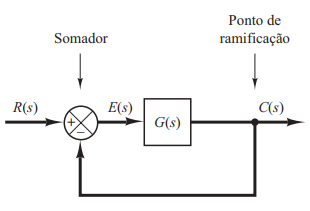
\includegraphics[scale=1]{figuras/closed_loop}
    \label{fig:closed_loop}
    \\
    \vspace{0cm}\hspace{0cm}\small{Fonte: \cite[Fig 2.3]{ogata2010engenharia}}
\end{figure}

Onde:
\begin{itemize}
    \item $R(s)$: Representa o sinal de referência.
    \item $G(s)$: Representa o sistema sistema.
    \item $C(s)$: Representa a saida.
    \item $E(s)$: É o erro ou a diferença entre $R(s)$ e $C(s)$.
\end{itemize}

\subsection{Modelo}\label{subsec:modelfund}

De acordo com \cite{CoelhoIdentificacao}, em controle de processos, um modelo não busca ser uma réplica exata do
sistema real, mas sim uma representação adequada para uma aplicação específica.
A modelagem é um procedimento que visa obter um conjunto de equações matemáticas que descrevem a dinâmica do sistema,
permitindo responder a questões sobre o sistema sem a realização de experimentações físicas.
A simplicidade é muitas vezes uma virtude na modelagem de processos, pois modelos excessivamente complexos podem
não ser necessários para capturar a dinâmica essencial do sistema para fins de controle.

A função de transferência é uma forma comum de representar o modelo de um sistema em controle de processos.
Ela é definida como a razão entre a transformada de Laplace da saída e da entrada do sistema,
sendo uma razão de dois polinômios em $s$, onde $s$ é a variável complexa da transformada de Laplace.
Esta representação é particularmente útil para a análise e o projeto de sistemas de controle,
pois permite uma avaliação clara da resposta do sistema a diferentes tipos de sinais de entrada,
como impulso, degrau, rampa e senoidal.

Um modelo clássico e comumente utilizado para representação de sistemas de controle de primeira ordem com atraso é
representado pela seguinte função de transferência:
\begin{equation}
    \label{eq:firstordertf}
    G(s) = \frac{K}{\tau s + 1}e^{-\theta s}
\end{equation}
onde cada termo tem um significado específico:
\begin{itemize}
    \item $G(s)$: Função de transferência do sistema no domínio da frequência.
    \item $K$: Ganho do sistema, que determina a amplitude da saída em relação à entrada.
    \item $\tau$: Constante de tempo do sistema, que indica a rapidez com que o sistema responde a uma entrada.
    \item $\theta$: Tempo de atraso, que representa o tempo que leva para a resposta do sistema começar após uma entrada.
    \item $s$: Variável complexa da Transformada de Laplace, usada para transformar funções do tempo para o domínio da frequência.
\end{itemize}

Este modelo é particularmente útil para descrever sistemas onde há um atraso perceptível entre a ação de controle e a
resposta observada.
A exponencial negativa \( e^{-\theta s} \) incorpora o atraso no modelo, deslocando a resposta do sistema no tempo.
A constante de tempo \( \tau \) e o ganho \( K \) são parâmetros fundamentais que influenciam a dinâmica do sistema.
Através de simulações baseadas neste modelo, é possível prever o comportamento do sistema sob diferentes
condições operacionais e ajustar o projeto de um controlador antes da implementação real.

No contexto da automação industrial, os modelos matemáticos são empregados para previsão, análise e projeto de sistemas
de controle, essenciais para a sintonia de controladores e a otimização de processos.

\subsection{Controlador}

Dentro do universo dos sistemas de controle, um controlador é um componente crucial que modula a entrada de um sistema
para alcançar a saída desejada.
Ele atua ajustando o sinal de controle em resposta às variações da saída, visando minimizar a diferença entre a saída
observada e a saída desejada, conhecida como sinal de referência.
Os controladores podem ser classificados de acordo com suas ações de controle, alguns exemplos são controladores,
como on-off, proporcionais, integrais, proporcional-integrais (PI), proporcional-derivativos (PD) e
proporcional-integral-derivativos (PID), cada um com características distintas que os tornam adequados para diferentes
aplicações industriais. \cite{ogata2010engenharia}.

%chck
O controlador PID é um dos tipos mais prevalentes de controladores em sistemas de controle, caracterizado pela sua
função de transferência,
\begin{equation}
    \label{eq:ctrlr}
    G_c(s) = K_p + \frac{K_i}{s} + K_d s
\end{equation}
onde \( K_p \), \( K_i \), e \( K_d \) representam os ganhos proporcional, integral e derivativo, respectivamente.
O termo proporcional \( K_p \) determina a reação do controlador à magnitude atual do erro,
o termo integral \( K_i \) acumula o erro ao longo do tempo, visando eliminar o erro estático,
e o termo derivativo \( K_d \) responde à taxa de variação do erro, antecipando o comportamento futuro.
A escolha adequada desses parâmetros é crucial: um \( K_p \) elevado pode acelerar a resposta do sistema, mas
potencialmente à custa da estabilidade;
um \( K_i \) excessivo pode introduzir oscilações devido ao atraso na resposta;
e um \( K_d \) significativo pode melhorar a estabilidade e a resposta rápida, mas é sensível ao ruído do sinal de
medição.
O ajuste dos três efeitos do controlador PID é essencial para otimizar o desempenho do sistema, tanto em resposta
transitória quanto em regime estacionário. \cite{ogata2010engenharia}.

Vale ressaltar que controladores como P, PI e PD, podem ser vistos como um controlador PID onde o ganho para os
parâmetros não citados é ajustado para zero.

\subsection{Métodos de Identificação}

Segundo \cite{CoelhoIdentificacao}, métodos de identificação de sistemas referem-se ao conjunto de técnicas
utilizadas para construir modelos matemáticos que capturam a dinâmica de sistemas reais a partir de dados de entrada e
saída.
Estes métodos buscam determinar os parâmetros do sistema que melhor se ajustam às medidas observadas,
permitindo que o modelo matemático reproduza o comportamento do sistema.
A identificação pode ser conduzida de duas formas principais: \textit{off-line} e \textit{on-line}.

Na identificação \textit{off-line}, coleta-se um conjunto de dados de entrada e saída, comumente referidos como dados discretos,
processados posteriormente para estimar os parâmetros do modelo.
Este processo não possui restrições de tempo computacional e é tipicamente realizado utilizando algoritmos
não-recursivos.
Já a identificação \textit{on-line} ajusta os parâmetros do modelo em tempo real, sem a necessidade de armazenar previamente as
medidas.
Utiliza-se um algoritmo recursivo que atualiza os parâmetros após cada amostra coletada,
o que é particularmente útil para sistemas que mudam com o tempo ou quando é necessário um ajuste contínuo do modelo.

Devido ao escopo deste trabalho, métodos de identificação \textit{on-line} não serão abordados, apenas métodos \textit{off-line} baseados
nos dados discretos de resposta do sistema.

\subsubsection{Ziegler Nichols}\label{subsubsec:znfun}

O método Ziegler-Nichols é um clássico da literatura para identificação de modelos dinâmicos de
processos industriais.
Desenvolvido por Ziegler e Nichols em 1942 \cite{CoelhoIdentificacao}.

O processo de identificação de um modelo por esse método envolve a análise da resposta de um sistema a um sinal
degrau, para obter os parâmetros da equação\eqref{eq:firstordertf}, $K$, $\tau$ e $\theta$ e criar
a função de transferência representativa do modelo do sistema analisado.

Os parâmetros são calculados conforme indicado pela figura a seguir:
\begin{figure}[H]
    \centering
    \caption{Métodos de ZN e HAG para a modelagem de processos de primeira ordem}
    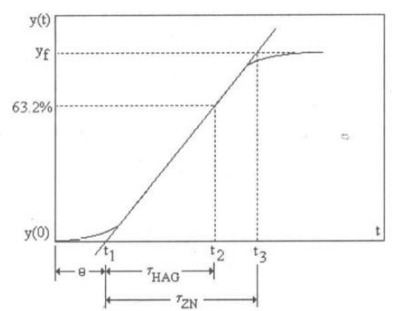
\includegraphics[scale=0.3]{figuras/zn_hg_ident_meth}
    \label{fig:zn_hg_ident_meth}
    \\
    \vspace{0cm}\hspace{0cm}\small{Fonte: \cite{CoelhoIdentificacao}}
\end{figure}

A reta traçada corresponde à tangente no ponto de máxima inclinação da curva de reação.

A constante de tempo $\tau$ é determinada pelo intervalo de tempo entre $t_1$, e o instante
$t_3$, onde a reta tangente toca o eixo $t$, e onde cruza com a reta $y(t) = y_f$,
respectivamente.
O valor de  $\theta$ é considerado como $t_1$, o intervalo entre a aplicação do sinal degrau e o
momento em que a reta tangente toca o eixo $t$.
Por fim o valor de $K$ pode ser obtido a través da equação,
\begin{equation}
    \label{eq:dydu}
    K = \frac{\Delta y}{\Delta u}
\end{equation}
Ou seja $y_f$ dividido pelo valor do sinal degrau. \cite{CoelhoIdentificacao}.

\subsubsection{Hagglund}

O método Hagglund é mais um clássico da literatura para identificação de modelos dinâmicos de
processos industriais.
Desenvolvido por Hagglund em 1991 \cite{CoelhoIdentificacao}.

A identificação de modelo pelo método de Hägglund é muito similar a de Ziegler e Nichols (\ref{subsubsec:znfun}), com a
única diferença sendo que $\tau$ é determinado pelo intervalo de tempo entre $t_1$, e o instante $t_2$, sendo $t_2$
o momento em que a curva de resposta alcança o valor $y(t) = y(0) + 0.632y_f$, ou seja $63.2\%$ do valor de regime.
Isso pode ser visualizado na figura \ref{fig:zn_hg_ident_meth}.

\subsubsection{Smith}\label{subsubsec:smfun}

Desenvolvido por Smith em 1985, o método Smith, assim como os métodos Hagglund e Ziegler-Nichols, busca encontrar
valores para os parâmetros $K$, $\tau$ e $\theta$ e criar a função de transferência representativa do modelo do sistema
analisado \cite{CoelhoIdentificacao}.

\begin{figure}[H]
    \centering
    \caption{Método de Smith para a modelagem de processos de primeira ordem}
    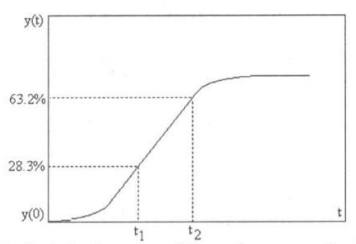
\includegraphics[scale=0.3]{figuras/sm_ident_meth}
    \label{fig:sm_ident_meth}
    \\
    \vspace{0cm}\hspace{0cm}\small{Fonte: \cite{CoelhoIdentificacao}}
\end{figure}

Na figura \ref{fig:sm_ident_meth} podem ser observados os momentos $t1$ e $t2$, eles correspondem a passagem da resposta
pelos pontos $y(t) = y(0) + 0.283y(\infty)$ e $y(t) = y(0) + 0.632y(\infty)$, respectivamente.

As constantes podem então ser utilizadas para o cálculo da constante de tempo $\tau$ e do valor de $\theta$,
conforme as seguintes equações:
\begin{equation}
    \label{eq:smtau}
    \tau = 1.5*(t_2 - t_1)
\end{equation}
\begin{equation}
    \label{eq:smtheta}
    \theta = t_2 - \tau
\end{equation}

Por fim o valor de $K$ pode ser obtido através da equação \eqref{eq:dydu}.

\subsubsection{Sundaresan Krishnaswamy}

O método de Sundaresan e Krishnaswamy, desenvolvido em 1977 é bastante similar ao método Smith \ref{subsubsec:smfun}.
Apresentando algumas alterações nos valores para o cácluculo das constantes de tempo $t1$ e $t2$, calculadas como
$y(t) = y(0) + 0.353y(\infty)$ e $y(t) = y(0) + 0.853y(\infty)$, respectivamente, como pode ser visto na figura
\ref{fig:sd_kr_ident_meth} \cite{CoelhoIdentificacao}:


\begin{figure}[H]
    \centering
    \caption{Método de Sundaresan e Krishnaswamy para a modelagem de processos de primeira ordem }
    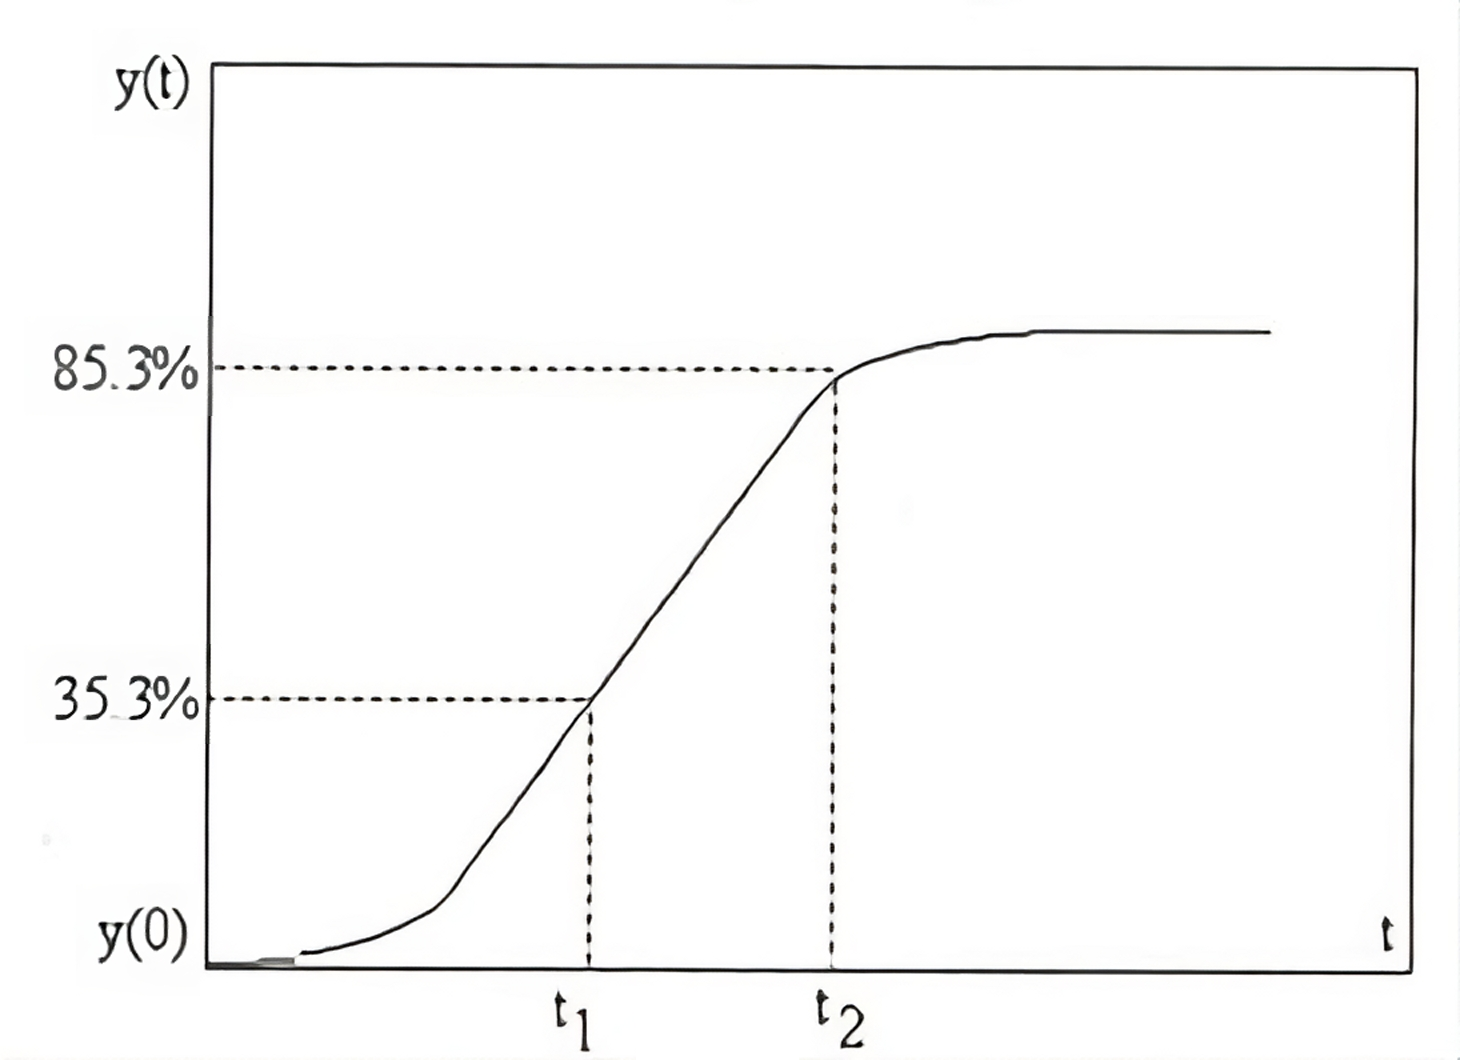
\includegraphics[scale=0.3]{figuras/sd_kr_ident_meth}
    \label{fig:sd_kr_ident_meth}
    \\
    \vspace{0cm}\hspace{0cm}\small{Fonte: \cite{CoelhoIdentificacao}}
\end{figure}

Além de ter diferenças nas equações de $\tau$ e $\theta$, como pode ser visto nas equações \eqref{eq:sktau} e
\eqref{eq:sktheta}:
\begin{equation}
    \label{eq:sktau}
    \tau = 0.67*(t_2 - t_1)
\end{equation}
\begin{equation}
    \label{eq:sktheta}
    \theta = 1.3t_1 - 0.29t_2
\end{equation}

\subsubsection{Nishikawa}

Um último um método clássico da literatura para Identificação de modelos é o desenvolvido por Nishikawa em 1984.
A pesar de buscar os mesmos parâmetros que os métodos anteriores, estes parâmetros são obtidos através de áreas
delimitadas pela curva de resposta a sinal degrau, pelo valor de regime e pela constante de tempo $t_0$, como pode ser
observado na figura \ref{fig:ni_ident_meth}.


\begin{figure}[H]
    \centering
    \caption{Método de Nishikawa para a modelagem de processos de primeira ordem}
    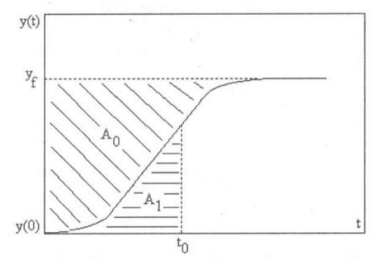
\includegraphics[scale=0.3]{figuras/ni_ident_meth}
    \label{fig:ni_ident_meth}
    \\
    \vspace{0cm}\hspace{0cm}\small{Fonte: \cite{CoelhoIdentificacao}}
\end{figure}

As áreas e a constante de tempo podem ser calculadas conforme as seguintes equações:

\begin{equation}
    \label{eq:nia0}
    A_0 = \int_{0}^{\infty} { \Delta y(\infty) - \Delta y(t) } dt
\end{equation}
\begin{equation}
    \label{eq:nia1nt0}
    A_1 = \int_{0}^{t_0} \Delta y(t) dt \;\; ; \;\; t_0 = \frac{A_0}{\Delta y(\infty)}
\end{equation}

Com isto, podem ser obtodas as constantes $\tau$ e $\theta$:
\begin{equation}
    \label{eq:nitau}
    \tau = \frac{A_1}{0.368\Delta y(\infty)}
\end{equation}
\begin{equation}
    \label{eq:nitheta}
    \theta = t_0 - \tau
\end{equation}

Da mesma forma que os outros métodos, $K$ pode ser obtido através da equação \eqref{eq:dydu}.

\subsection{Métodos de Aproximação de Controlador PID}

A sintonia de controladores PID é um componente crucial no desenvolvimento de sistemas de controle automatizados,
fundamental para assegurar a eficiência e a estabilidade operacional.
A importância da sintonia reside na sua capacidade de ajustar o comportamento do sistema de controle para atender às
especificações de desempenho, como precisão, rapidez de resposta e estabilidade a longo prazo.
A sintonia adequada consegue compensar as incertezas inerentes ao modelo do sistema e as variações ambientais,
garantindo que o sistema mantenha seu desempenho ótimo sob uma gama de condições operacionais.
\cite{apostpidsint}.

Realizar a sintonia de um controlador PID envolve a aproximação dos ganhos do controlador capazes de causar o efeito no
sistema.
Para isso é comumente feita a análise o modelo do sistema a ser controlado.
Através da análise do modelo, é possível prever como o sistema responde a diferentes configurações de controle e
identificar os parâmetros de ganho que resultarão na resposta desejada.
Este processo de aproximação dos ganhos, permite a sintonia do sistema, assegurando que o controlador PID opere de forma
eficiente, mantendo a saída do sistema nos parâmetros desejados, minimizando o erro e otimizando a resposta a
perturbações. \cite{apostpidsint}.

\subsubsection{Ziegler Nichols}\label{subsubsec:znctr}

Proposto por Ziegler e Nichols, como uma forma de obter os ganhos de controlador para os modelos itentificados
pelo seu método de indentificação (\ref{subsubsec:znfun}), o objetivo deste método é obter parâmetros de ganho PID que
façam a sintonia do controlador \cite{apostpidsint}.

Em espessífico, este método se baseia na curva de reação do sistema a resposta de sinal degrau, que é
exatamente o que o resultado da identificação por Ziegler Nichols obtém, utilizando os parâmetros $K$, $\tau$ e $\theta$
para análise.

Desta forma, são aplicadas as fórmulas do método de acordo com a tabela \ref{tab:zncntb}.

\begin{table}[h]
    \begin{center}
        \begin{tabular}{ | l | c | c | c | }
            \hline
            {\textbf{Controlador}} & {$K_P$}                               & {$T_I$}                & {$T_D$}       \\
            \hline
            {\textbf{P}}           & {$\frac{1}{K}\frac{\tau}{\theta}$}    & {$\infty$}             & {$0$}         \\
            \hline
            {\textbf{PI}}          & {$0.9\frac{1}{K}\frac{\tau}{\theta}$} & {$\frac{\theta}{0.3}$} & {$0$}         \\
            \hline
            {\textbf{PID}}         & {$1.2\frac{1}{K}\frac{\tau}{\theta}$} & {$2\theta$}            & {$0.5\theta$} \\
            \hline
        \end{tabular}
        \caption{Método de Ziegler e Nichols para Curva de Reação}
        \label{tab:zncntb}
    \end{center}
\end{table}

Os valores de $T_I$ e $T_D$ são $1/K_i$ e $1/K_d$, respectivamente.

\subsubsection{Cohen Coon}

Criado por Cohen e Coon como uma forma de obter os ganhos de controlador, de forma similar ao método de Ziegler e Nichols
(\ref{subsubsec:znctr}), para modelos clássicos de primeira ordem com atraso.
Utiliza a seguinte tabela para determinar os ganhos de controlador PID:

\begin{table}[h]
    \begin{center}
        \begin{tabular}{ | l | c | c | c | }
            \hline
            {\textbf{Controlador}} & {$K_P$}                               & {$T_I$}                & {$T_D$}       \\
            \hline
            {\textbf{P}}           & {$\frac{1}{K}\frac{\tau}{\theta}[1+\frac{\theta}{3\tau}]$}    & {$\infty$}             & {$0$}         \\
            \hline
            {\textbf{PI}}          & {$\frac{1}{K}\frac{\tau}{\theta}[0.9+\frac{\theta}{12\tau}]$} & {$\frac{\theta [30+3 \frac{\theta}{\tau}]}{9+20 \frac{\theta}{\tau}}$} & {$0$}         \\
            \hline
            {\textbf{PID}}         & {$\frac{1}{K}\frac{\tau}{\theta}[\frac{16\tau+3\theta}{12\tau}]$} & {$\frac{\theta [32+6 \frac{\theta}{\tau}]}{13+8 \frac{\theta}{\tau}}$}            & {$\frac{4 \theta}{11+2 \frac{\theta}{\tau}}$} \\
            \hline
        \end{tabular}
        \caption{Método de Cohen e Coon para Curva de Reação}
        \label{tab:cccntb}
    \end{center}
\end{table}

Os valores de $T_I$ e $T_D$ são $1/K_i$ e $1/K_d$, respectivamente.

\section{Implementação em {Python}}

\subsection{Bibliotecas em {Python}}

No ecossistema de programação {Python}, bibliotecas desempenham um papel fundamental, servindo como repositórios ricos de
funções e métodos pré-construídos que permitem aos desenvolvedores executar uma gama ampla de tarefas com eficiência e
precisão.
Essas bibliotecas podem variar em seu escopo e aplicação, abrangendo desde operações matemáticas complexas, como as
oferecidas pelo NumPy, até a manipulação avançada de dados com o pandas, e interações de rede simplificadas através da
biblioteca requests.
A habilidade de reutilizar e adaptar código pré-existente não apenas acelera o processo de desenvolvimento, mas também
assegura a adesão a padrões de código testados e confiáveis \cite{pipy,pydocs} .

A ferramenta pip e o Python Package Index (PyPI) são componentes centrais na gestão e instalação de bibliotecas {Python}.
O pip, recomendado pela {Python} Packaging Authority (PyPA), é essencial para a instalação de pacotes {Python},
facilitando a integração de bibliotecas de terceiros em projetos de desenvolvimento.
Por meio do pip, os usuários podem instalar pacotes diretamente do PyPI, um vasto repositório que hospeda milhares de
pacotes criados pela comunidade {Python} global.
Essa centralização de recursos no PyPI, acessível via pip, não apenas proporciona uma plataforma unificada para a
distribuição de software, mas também simplifica significativamente o gerenciamento de dependências em projetos de
{Python}.
O uso combinado de pip e PyPI é uma prática padrão no desenvolvimento Python, garantindo que os desenvolvedores tenham
acesso fácil a uma ampla gama de ferramentas e bibliotecas \cite{pip}.

\subsection{Documentação de código}

A documentação de código é uma parte essencial do desenvolvimento de software, especialmente em linguagens dinâmicas e
flexíveis como Python.
Uma boa documentação não apenas facilita a compreensão e o uso do código por outros desenvolvedores, mas também serve
como uma referência valiosa para o autor durante manutenções e atualizações futuras.
Em Python, a documentação eficaz geralmente inclui docstrings detalhadas para funções, classes e módulos, além de
comentários explicativos no código.
Essas práticas de documentação são fundamentais para garantir a legibilidade e a manutenção do código, permitindo que
outros desenvolvedores e usuários compreendam rapidamente a finalidade e o funcionamento das diversas partes do software
\cite{pydocs}.

Sphinx é uma ferramenta robusta e versátil para a criação de documentação, amplamente utilizada na comunidade Python.
Ela transforma docstrings escritas em reStructuredText em uma variedade de formatos de saída ricos, incluindo HTML,
LaTeX, man pages e outros.
O Sphinx é particularmente conhecido por sua capacidade de gerar automaticamente documentação a partir do código-fonte,
além de suportar a escrita de documentação extensiva separadamente.
Esta ferramenta desempenha um papel crucial na manutenção de documentações claras e atualizadas, essencial para projetos
de software de qualquer escala, especialmente em ambientes colaborativos e de código aberto \cite{sphinx}.

Complementando as ferramentas de documentação como o Sphinx, plataformas como o Read the Docs oferecem um serviço de
hospedagem para documentações de software.
O Read the Docs simplifica o processo de publicação e atualização de documentações, integrando-se diretamente com
repositórios de código como GitHub, GitLab e Bitbucket.
Ele automatiza a construção e atualização da documentação sempre que o código-fonte é atualizado, garantindo que a
documentação permaneça sincronizada com as versões mais recentes do software.
Esta plataforma é amplamente adotada em projetos de código aberto, proporcionando aos desenvolvedores uma maneira
eficiente e eficaz de manter suas documentações acessíveis e atualizadas para usuários e colaboradores \cite{rtd}.

\subsection{Controle em Python}

A biblioteca de controle Python, conhecida como \textit{Python Control Systems Library}, é uma ferramenta muito útil no campo da
engenharia de controle.
Ela oferece uma gama de funcionalidades para análise e projeto de sistemas de controle.
Esta biblioteca é projetada para ser compatível com as convenções e práticas de controle já estabelecidas, facilitando
a transição para aqueles que já estão familiarizados com ferramentas de controle tradicionais como MATLAB.
A Python Control Systems Library inclui recursos para a modelagem de sistemas dinâmicos, análise de resposta em
frequência, projeto de controladores, entre outras funcionalidades essenciais no estudo e aplicação de sistemas de
controle.
A utilização desta biblioteca em ambientes educacionais e profissionais tem se mostrado cada vez mais prevalente,
devido à sua eficiência e capacidade de integração com outras ferramentas Python para cálculos numéricos e análise de
dados \cite{ctrlib}.

A bibliotéca possui uma documentação extensiva, oferecendo uma visão abrangente das capacidades da biblioteca,
com exemplos e tutoriais detalhados.

\subsection{Outras Bibliotecas}

\subsubsection{NumPy}

NumPy é uma biblioteca essencial para a computação científica em Python, oferecendo suporte para grandes arrays e
matrizes multidimensionais, juntamente com uma vasta coleção de funções matemáticas de alto nível para operar nessas
estruturas de dados.
É a base sobre a qual muitas outras bibliotecas científicas e de análise de dados, incluindo Pandas, são construídas.
NumPy é especialmente valorizado por sua eficiência em cálculos numéricos, devido à sua implementação por trás dos panos
em linguagens de baixo nível como C e Fortran.
Isso permite que operações que seriam lentas em Python puro sejam executadas de maneira muito mais rápida.
A biblioteca é amplamente utilizada em diversas áreas que requerem cálculos numéricos e análise de dados, incluindo
engenharia, física, estatística e machine learning \cite{numpy}.

\subsubsection{Pandas}

Pandas é uma biblioteca escrita para Python, focada na manipulação e análise de dados.
Ela oferece estruturas de dados e operações para manipular tabelas numéricas e séries temporais, tornando-se uma
ferramenta indispensável na ciência de dados e em aplicações analíticas.
A biblioteca é construída sobre o NumPy e torna a análise de dados complexos acessível e eficiente, com estruturas como
DataFrame e Series.
A biblioteca facilita tarefas como a leitura de dados de várias fontes, limpeza de dados, transformações, e visualização
de dados \cite{pandas}.

\subsubsection{SymPy}

SymPy é uma biblioteca de matemática simbólica para Python, utilizada para realizar computações simbólicas em vez de
numéricas.
Isso significa que, com o SymPy, é possível manipular expressões matemáticas exatamente, em vez de aproximá-las
numericamente.
A biblioteca permite a execução de tarefas como a simplificação de expressões, cálculo de derivadas, integrais e
limites, solução de equações, manipulação de algebra linear, entre outras operações simbólicas.
O SymPy é especialmente útil em contextos educacionais e de pesquisa, onde a precisão das expressões matemáticas é
crucial.
Sua natureza simbólica o torna uma ferramenta valiosa para a verificação analítica de soluções, exploração matemática e
ensino de conceitos matemáticos \cite{sympy}.

\subsubsection{Matplotlib}

Matplotlib é uma biblioteca de plotagem, amplamente usada na comunidade científica e analítica, ela permite a criação de
gráficos e visualizações de dados em 2D e 3D de alta qualidade.
É conhecida pela sua flexibilidade e capacidade de gerar uma ampla variedade de gráficos e diagramas, incluindo
histogramas, gráficos de dispersão, gráficos de linhas, gráficos de área, barras de erro, boxplots, entre outros.
A biblioteca é altamente personalizável e pode ser usada em \textit{scripts Python}, \textit{shell Python} e Jupyter,
interfaces gráficas de aplicativos e servidores de aplicativos da ‘web’.
Sua capacidade de integrar-se bem com muitas plataformas de desenvolvimento e sua interface semelhante ao MATLAB tornam
ela uma escolha popular para visualização de dados, análise exploratória de dados e apresentação de resultados
científicos \cite{matplotlib}.

\subsection{Ferramentas Auxiliares ao Desenvolvimento}

\subsubsection{Controle de Versão}

\abreviatura{CI/CD}{Integração Contínua e Entrega Contínua}

O controle de versão é uma prática essencial no desenvolvimento de software, e o Git é uma das ferramentas mais
populares e poderosas nesse domínio.
Git é um sistema de controle de versão distribuído que facilita o rastreamento de mudanças em arquivos e coordena o
trabalho entre múltiplos colaboradores.
Ele permite que desenvolvedores criem \textit{branches} para desenvolver funcionalidades ou testar ideias em ambientes
isolados, sem afetar o código principal.
Além disso, o Git oferece robustas funcionalidades de \textit{merge} para integrar diferentes linhas de desenvolvimento
\cite{git}.

GitHub, é uma plataforma baseada no Git, mas que adiciona novas funcionalidades ao controle de versão, oferecendo uma
interface \textit{web} rica e uma série de recursos para colaboração em projetos de software.
Além de hospedar repositórios Git, ele também fornece ferramentas para revisão de código, gerenciamento de projetos,
integração contínua e entre outras.
Uma das funcionalidades notáveis do GitHub é o GitHub Actions, um recurso de CI/CD que automatiza fluxos de trabalho
de software.
Com GitHub Actions, os desenvolvedores podem criar \textit{pipelines} personalizados para testar, construir e implantar
aplicações diretamente no GitHub, facilitando a automação de processos e a entrega contínua de software \cite{github}.

\subsubsection{Mypy}
Mypy é uma ferramenta importante no ecossistema Python, oferecendo suporte à checagem de tipos estáticos.
Ele permite que os desenvolvedores adicionem anotações de tipo ao seu código, sendo então verificadas pelo Mypy para
erros de tipo em tempo de compilação.
Isso ajuda a garantir programas corretos e a prevenir \textit{bugs} relacionados a tipos, especialmente em bases de
código maiores ou mais complexas \cite{mypy}.

\subsubsection{Flake8}

Flake8 é uma ferramenta de verificação de código para Python, que combina PyFlakes, pycodestyle (anteriormente conhecido
como pep8), e Ned Batchelder’s McCabe script.
Ela verifica o código-fonte contra erros de programação, estilos inconsistentes e construções complexas ou duvidosas.
Ao aderir ao PEP 8, as diretrizes de estilo do Python, o Flake8 ajuda a manter a legibilidade e a consistência do
código \cite{flake8}.

\subsubsection{Pytest}

Pytest é um \textit{framework} de testes para Python, conhecido por sua simplicidade, escalabilidade e capacidade de
suportar testes simples e complexos.
Ele permite escrever testes de forma rápida e organizada, com suporte a \textit{fixtures} e \textit{plugins} que podem
estender ainda mais suas funcionalidades.
Pytest torna os testes mais expressivos e fáceis de escrever, com uma sintaxe simples e a capacidade de executar testes
em paralelo, acelerando o processo de teste.
A ferramenta é uma escolha popular entre desenvolvedores Python para testes unitários, testes de integração e até mesmo
testes de sistema devido à sua flexibilidade e capacidade \cite{pytest}.

\subsubsection{Tox}

Tox é uma ferramenta para automação de testes em ambientes virtuais Python, facilitando o teste de pacotes em múltiplas
versões do Python.
Ele cria ambientes de teste isolados, onde pode-se testar a compatibilidade do código com diferentes versões do Python
e dependências de terceiros.
Tox é amplamente usado em projetos Python para automação de testes e integração contínua, garantindo que o software
funcione conforme esperado em vários ambientes e configurações \cite{tox}.


\chapter{Desenvolvimento}
Neste capítulo são apresentados a metodologia e detalhes sobre o desenvolvimento do trabalho.
Nos itens deste capítulo será apresentada a metodologia e detalhado o desenvolvimento do software da biblioteca,
demonstrando requisitos, arquitetura, ambiente de implementação, documentação e implementação.


\section{Metodologia}
topico pequeno enchendo linguiça


\section{Requisitos da Biblioteca}

O levantamento de requisitos e concepção inicial da dinâmica e uso da biblioteca, foi realizado com base no caminho de
acesso as funcionalidades que um usuário da biblioteca faria, de forma a levar em conta os objetivos específicos
propostos na introdução do trabalho.

O resultado da análise foi o seguinte diagrama de casos de uso, que denota um caminho provável de ações do usuário:

\begin{figure}[H]
    \centering
    \caption{Casos de uso}
    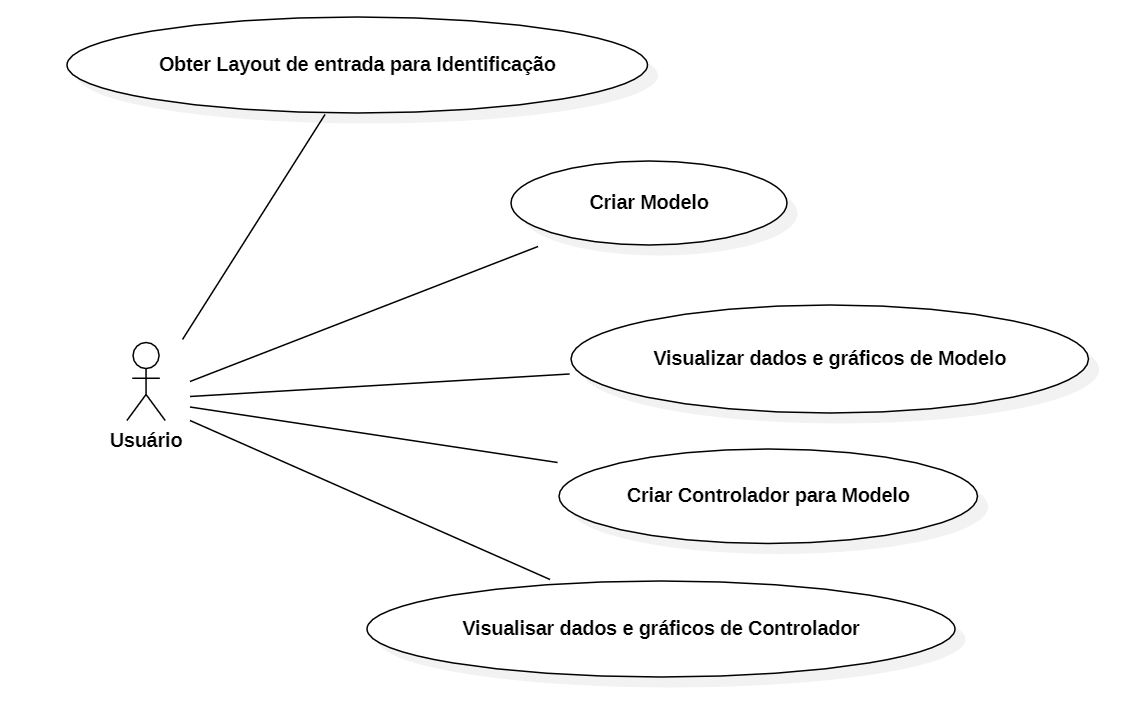
\includegraphics[scale=0.5]{figuras/use_cases}
    \label{fig:use_cases}
    \\
    \vspace{0cm}\hspace{0cm}\small{Fonte: Do autor}
\end{figure}

As tabelas \ref{tab:uc1}, \ref{tab:uc2}, \ref{tab:uc3}, \ref{tab:uc4}, \ref{tab:uc5} detalham os casos de uso ilustrado
na figura \ref{fig:use_cases}, especificando o objetivo, os pré requisitos e o cenário de cada caso de uso.


\begin{table}[!htbp]
    \begin{center}
        \begin{tabularx}{\textwidth}{|>{\bfseries\raggedright\arraybackslash\center}m{5cm}|X|}
            \hline
            Identificador UC: UC-1\newline Diagrama ID: D-1 & Nome: Obtenção de layout de input de dados para identificação\newline Prioridade: Alta                                                                                                                                                                                                   \\ \hline
            Objetivo                                        & Fornecer planilha de layout para que sejam inseridos os dados necessários para um determinado processo de identificação.                                                                                                                                                                 \\ \hline
            Atores                                          & Usuário                                                                                                                                                                                                                                                                                  \\ \hline
            Restrições                                      & Deve-se salvar a planilha referente ao layout necessário.                                                                                                                                                                                                                                \\ \hline
            Pré-condições                                   & -                                                                                                                                                                                                                                                                                        \\ \hline
            Cenário principal                               & 1. O método é chamado, recebendo o caminho onde deve salvar o arquivo e possívelmente os parâmetros referentes ao layout em espessífico, como tipo de arquivo, por exemplo.\newline 2. É construido em memória o layout desejado.\newline 3. É salvo o arquivo no caminho espessificado. \\ \hline
            Pós condições                                   & O Usuário possui o layout e pode inserir os dados.                                                                                                                                                                                                                                       \\ \hline
        \end{tabularx}
        \caption{Obtenção de layout de input de dados para identificação}
        \label{tab:uc1}
    \end{center}
\end{table}

\begin{table}[!htbp]
    \begin{center}
        \begin{tabularx}{\textwidth}{|>{\bfseries\raggedright\arraybackslash\center}m{5cm}|X|}
            \hline
            Identificador UC: UC-2\newline Diagrama ID: D-2 & Nome: Indentificação de sistema\newline Prioridade: Alta                                                                                                                                                                                                                                             \\ \hline
            Objetivo                                        & Realizar processo de identificação do sistema baseado nos dados e obter modelo.                                                                                                                                                                                                                      \\ \hline
            Atores                                          & Usuário                                                                                                                                                                                                                                                                                              \\ \hline
            Restrições                                      & Deve-se obter o modelo do sistema.                                                                                                                                                                                                                                                                   \\ \hline
            Pré-condições                                   & layout de dados preenchido.                                                                                                                                                                                                                                                                          \\ \hline
            Cenário principal                               & 1. O método de identificação é chamado, recebendo o caminho do arquivo de layout e possívelmente os parâmetros referentes ao método em espessífico.\newline 2. São realizados os cálculos e é obtido o objeto de modelo do sistema.\newline 3. O objeto de modelo do sistema é retornado ao usuário. \\ \hline
            Pós condições                                   & O Usuário possui um objeto de modelo do sistema.                                                                                                                                                                                                                                                     \\ \hline
        \end{tabularx}
        \caption{Indentificação de sistema}
        \label{tab:uc2}
    \end{center}
\end{table}

\begin{table}[!htbp]
    \begin{center}
        \begin{tabularx}{\textwidth}{|>{\bfseries\raggedright\arraybackslash\center}m{5cm}|X|}
            \hline
            Identificador UC: UC-3\newline Diagrama ID: D-3 & Nome: Visualização de modelo de sistema\newline Prioridade: Alta                                                                                                                                                                                                                         \\ \hline
            Objetivo                                        & Visualizar gráfico e dados indicadores importantes de um modelo.                                                                                                                                                                                                                         \\ \hline
            Atores                                          & Usuário                                                                                                                                                                                                                                                                                  \\ \hline
            Restrições                                      & Deve ser possível visualisar gráfico e dados indicadores importantes do modelo.                                                                                                                                                                                                          \\ \hline
            Pré-condições                                   & O Usuário possui um objeto de modelo do sistema.                                                                                                                                                                                                                                         \\ \hline
            Cenário principal                               & 1. Um método de visualisação de dados ou gráfico é chamado, passando possíveis parâmetros necessários ou que irão mudar a forma como os dados serão exibidos.\newline 2. São preparados os objetos a serem exibidos ao usuário.\newline 3. São exibidos os dados ou gráficos ao usuário. \\ \hline
            Pós condições                                   & O Usuário pode visualisar os dados do modelo.                                                                                                                                                                                                                                            \\ \hline
        \end{tabularx}
        \caption{Visualização de modelo de sistema}
        \label{tab:uc3}
    \end{center}
\end{table}

\begin{table}[!htbp]
    \begin{center}
        \begin{tabularx}{\textwidth}{|>{\bfseries\raggedright\arraybackslash\center}m{5cm}|X|}
            \hline
            Identificador UC: UC-4\newline Diagrama ID: D-4 & Nome: Aproximação de Controlador baseado em modelo de sistema\newline Prioridade: Alta                                                                                                                                                                                                     \\ \hline
            Objetivo                                        & Obter aproximação de parâmetros de controle baseados no modelo obtido.                                                                                                                                                                                                                     \\ \hline
            Atores                                          & Usuário                                                                                                                                                                                                                                                                                    \\ \hline
            Restrições                                      & Deve-se obter uma aproximação dos parâmetros do controlador.                                                                                                                                                                                                                               \\ \hline
            Pré-condições                                   & O Usuário possui um objeto de modelo do sistema.                                                                                                                                                                                                                                           \\ \hline
            Cenário principal                               & 1. O método de aproximação é chamado, recebendo o modelo do sistema e possívelmente os parâmetros referentes ao método de aproximação em espessífico.\newline 2. São realizados os cálculos e é obtido o objeto de controlador.\newline 3. O objeto de controlador é retornado ao usuário. \\ \hline
            Pós condições                                   & O Usuário possui um objeto de controlador.                                                                                                                                                                                                                                                 \\ \hline
        \end{tabularx}
        \caption{Aproximação de Controlador baseado em modelo de sistema}
        \label{tab:uc4}
    \end{center}
\end{table}

\begin{table}[!htbp]
    \begin{center}
        \begin{tabularx}{\textwidth}{|>{\bfseries\raggedright\arraybackslash\center}m{5cm}|X|}
            \hline
            Identificador UC: UC-5\newline Diagrama ID: D-5 & Nome: Visualização de controlador\newline Prioridade: Alta                                                                                                                                                                                                                               \\ \hline
            Objetivo                                        & Visualizar gráfico e dados indicadores importantes de um controlador.                                                                                                                                                                                                                    \\ \hline
            Atores                                          & Usuário                                                                                                                                                                                                                                                                                  \\ \hline
            Restrições                                      & Deve ser possível visualisar gráfico e dados indicadores importantes do controlador gerado.                                                                                                                                                                                              \\ \hline
            Pré-condições                                   & O Usuário possui um objeto de controlador.                                                                                                                                                                                                                                               \\ \hline
            Cenário principal                               & 1. Um método de visualisação de dados ou gráfico é chamado, passando possíveis parâmetros necessários ou que irão mudar a forma como os dados serão exibidos.\newline 2. São preparados os objetos a serem exibidos ao usuário.\newline 3. São exibidos os dados ou gráficos ao usuário. \\ \hline
            Pós condições                                   & O Usuário pode visualisar os dados do controlador.                                                                                                                                                                                                                                       \\ \hline
        \end{tabularx}
        \caption{Visualização de controlador}
        \label{tab:uc5}
    \end{center}
\end{table}




\section{Descrição da arquitetura}\label{sec:descarc}

A fim de construir uma biblioteca com arquitetura de código compreensível e escalável, optou-se pela orientação
da mesma a classes e objetos.
Baseado nisso e nos casos de uso, foi desenvolvido o diagrama de classes da figura \ref{fig:class_diag}.
Onde foram definidas as seguintes classes:
\begin{alineas}
    \item \textbf{DataInputUtils}: Classe utilitária para a entrada de dados externos - pode ser melhor visualizada na figura \ref{fig:class_diag_diubmi};
    \item \textbf{DataUtils}: Classe utilitária para manipulação de dados em memória - pode ser melhor visualizada na figura \ref{fig:class_diag_dupu};
    \item \textbf{PlotUtils}: Classe utilitária para plot de funções de transferência e outras informações relacionadas - pode ser melhor visualizada na figura \ref{fig:class_diag_dupu};
    \item \textbf{Model}: Classe representativa do Modelo matemático de uma planta de sistemas de controle - pode ser melhor visualizada na figura \ref{fig:class_diag_model};
    \item \textbf{ModelView}: Classe utilizada pra visualização de dados de um objeto da classe Model - pode ser melhor visualizada na figura \ref{fig:class_diag_model};
    \item \textbf{BaseModelIdentification}: Classe utilitária base para Identificação de modelos (Model), herdada por classes que implementam métodos de identificação - pode ser melhor visualizada na figura \ref{fig:class_diag_diubmi};
    \item \textbf{Controller}: Classe representativa do Modelo matemático de uma planta de sistemas de controle em Malha Fechada com Controlador PID - pode ser melhor visualizada na figura \ref{fig:class_diag_controller};
    \item \textbf{ControllerView}: Classe utilizada pra visualização de dados de um objeto da classe Controller - pode ser melhor visualizada na figura \ref{fig:class_diag_controller};
    \item \textbf{BaseControllerAproximation}: Classe utilitária base para aproximação de controladores (Controller), herdada por classes que implementam métodos de aproximação de parâmetros de controlador PID - pode ser melhor visualizada na figura \ref{fig:class_diag_bcacontroller}.
\end{alineas}

\begin{figure}[H]
    \centering
    \caption{Diagrama de classes}
    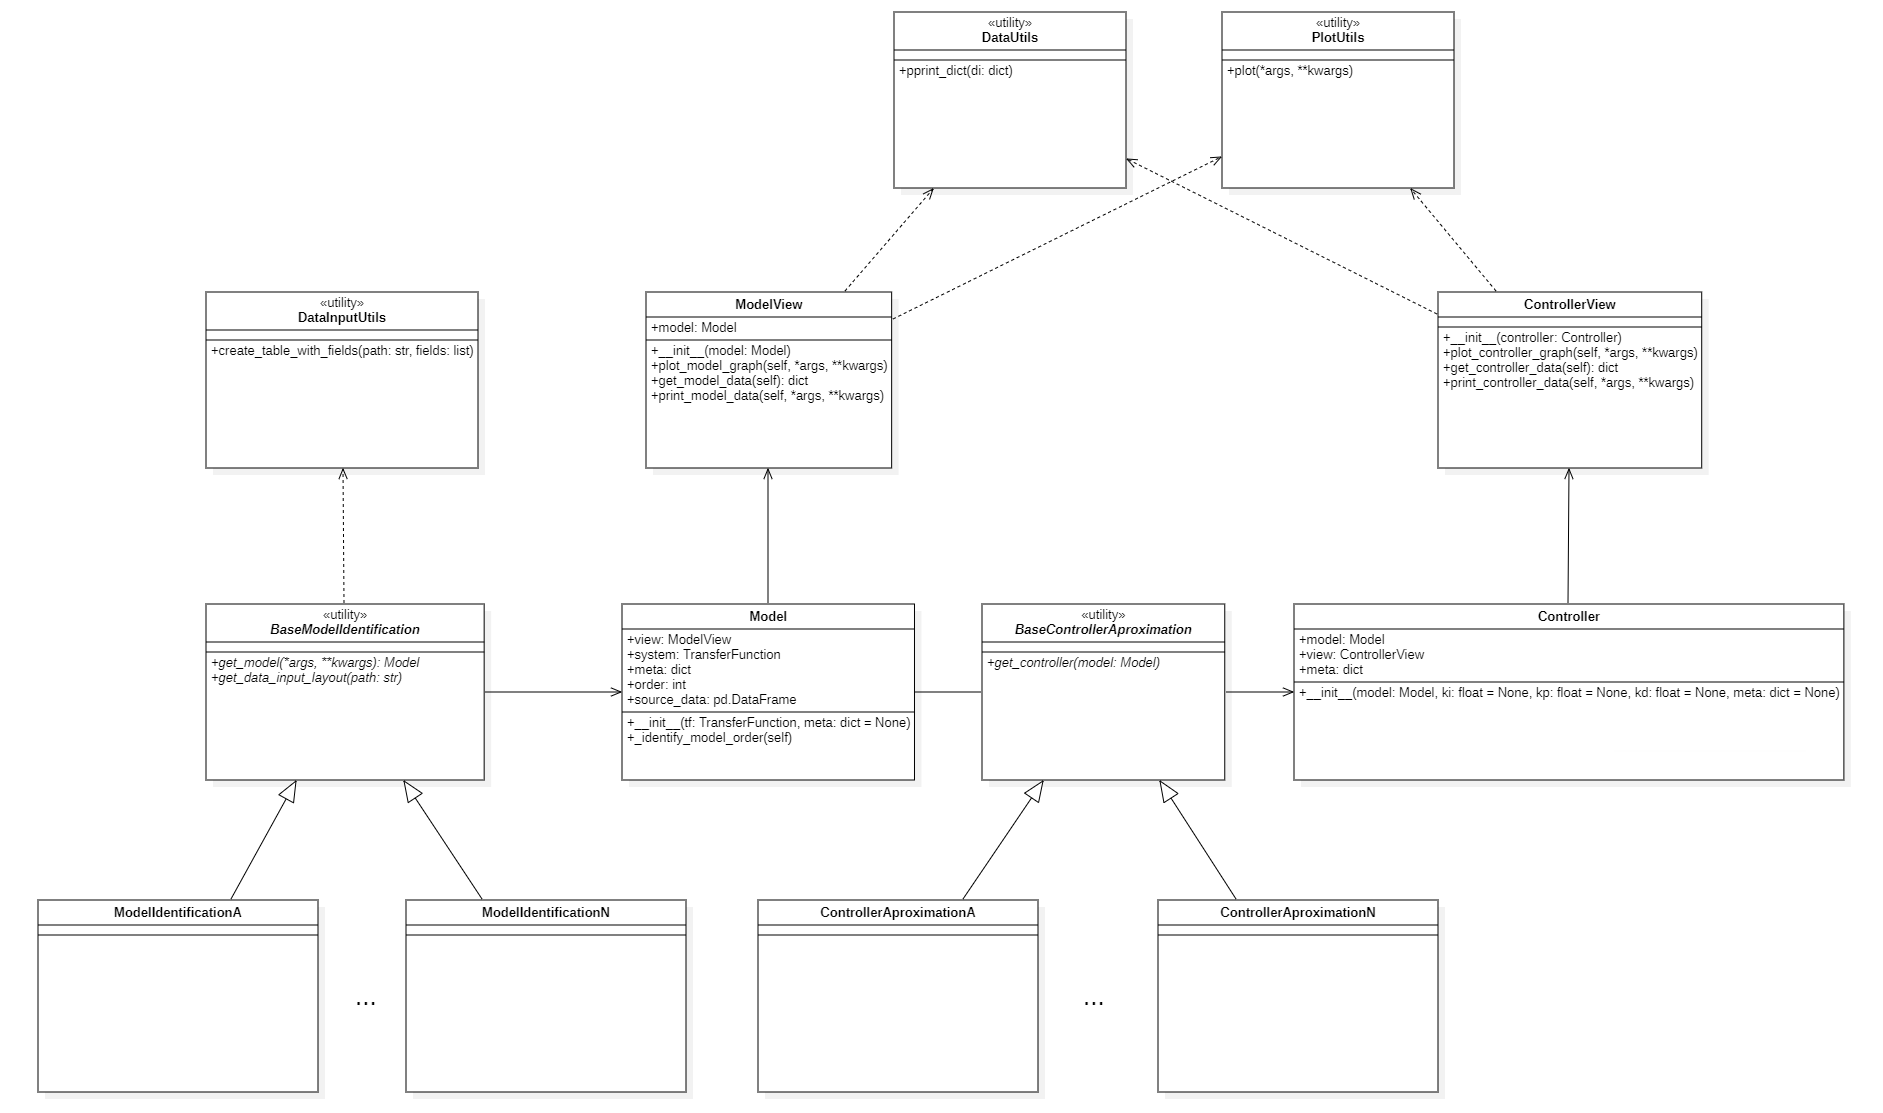
\includegraphics[scale=0.32]{figuras/class_diag}
    \label{fig:class_diag}
    \\
    \vspace{0cm}\hspace{0cm}\small{Fonte: Do autor}
\end{figure}

\begin{figure}[H]
    \centering
    \caption{Diagrama de classes ampliado - DataInputUtils e BaseModelIdentification}
    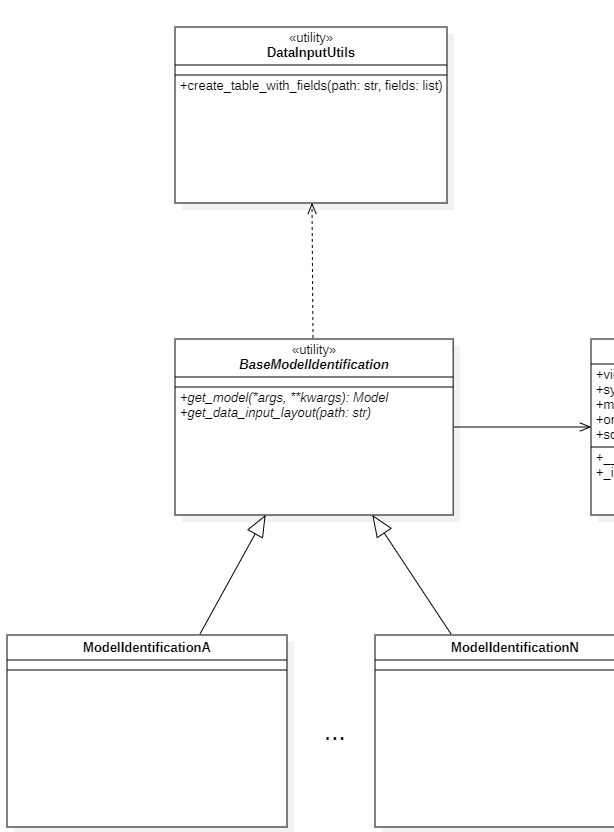
\includegraphics[scale=0.6]{figuras/class_diag_diubmi}
    \label{fig:class_diag_diubmi}
    \\
    \vspace{0cm}\hspace{0cm}\small{Fonte: Do autor}
\end{figure}

\begin{figure}[H]
    \centering
    \caption{Diagrama de classes ampliado - DataUtils e PlotUtils}
    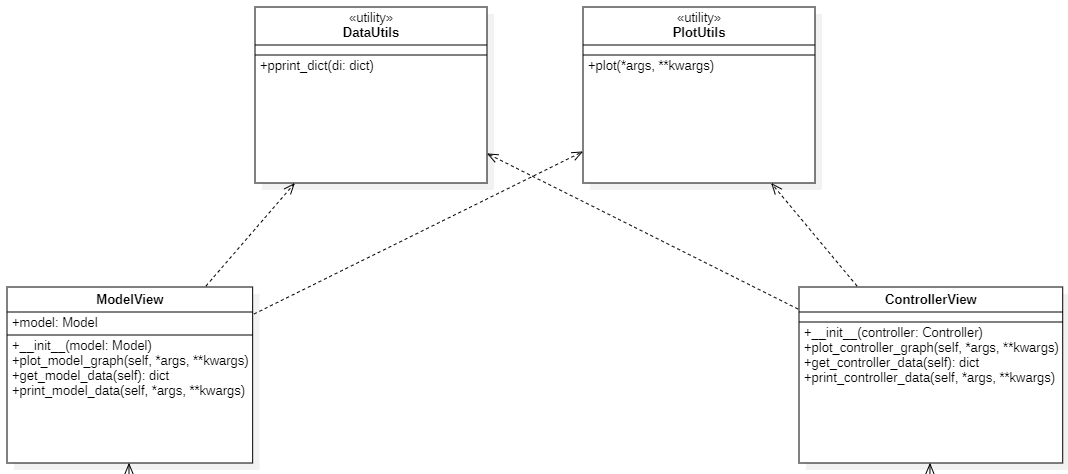
\includegraphics[scale=0.6]{figuras/class_diag_dupu}
    \label{fig:class_diag_dupu}
    \\
    \vspace{0cm}\hspace{0cm}\small{Fonte: Do autor}
\end{figure}

\begin{figure}[H]
    \centering
    \caption{Diagrama de classes ampliado - Model e ModelView}
    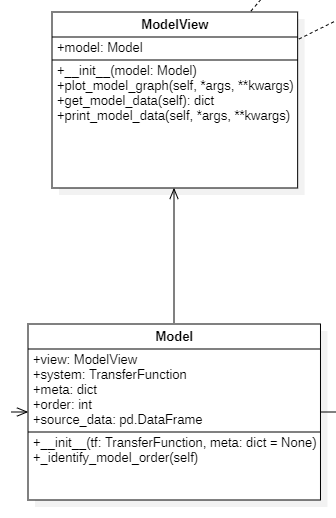
\includegraphics[scale=0.7]{figuras/class_diag_model}
    \label{fig:class_diag_model}
    \\
    \vspace{0cm}\hspace{0cm}\small{Fonte: Do autor}
\end{figure}

\begin{figure}[H]
    \centering
    \caption{Diagrama de classes ampliado - Controller e ControllerView}
    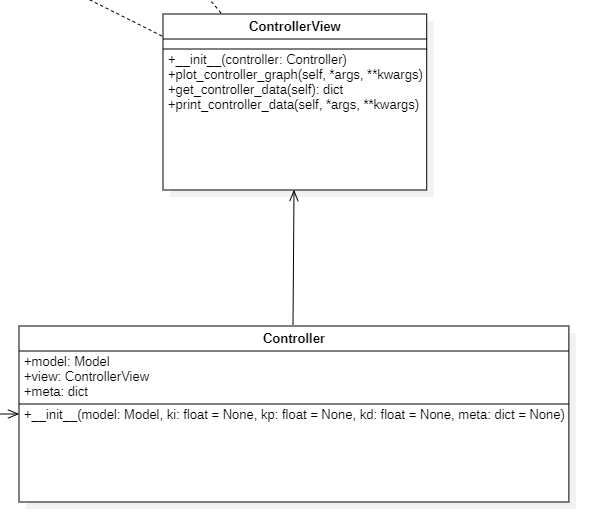
\includegraphics[scale=0.7]{figuras/class_diag_controller}
    \label{fig:class_diag_controller}
    \\
    \vspace{0cm}\hspace{0cm}\small{Fonte: Do autor}
\end{figure}

\begin{figure}[H]
    \centering
    \caption{Diagrama de classes ampliado - BaseControllerAproximation}
    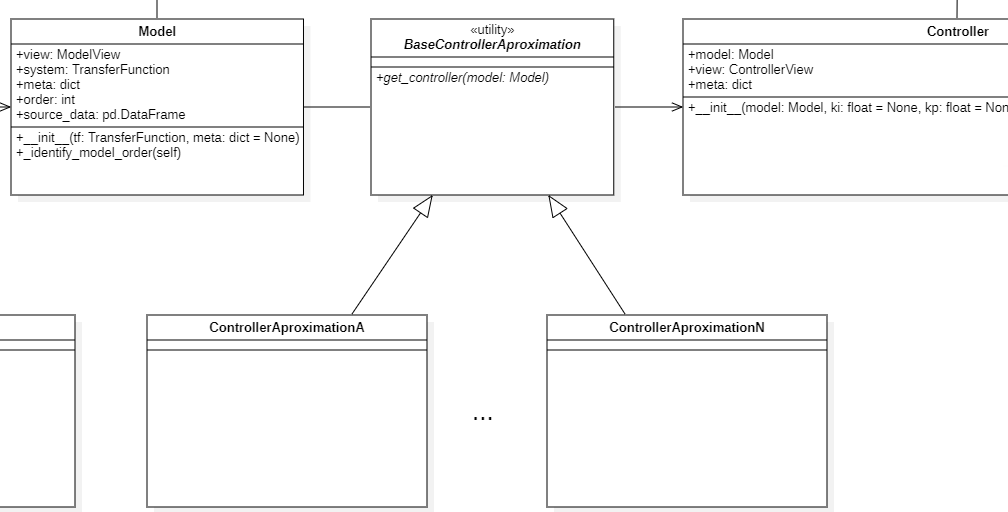
\includegraphics[scale=0.6]{figuras/class_diag_bcacontroller}
    \label{fig:class_diag_bcacontroller}
    \\
    \vspace{0cm}\hspace{0cm}\small{Fonte: Do autor}
\end{figure}

\section{Descrição do ambiente de implementação}

Nesta sessão serão explorados itens referentes ao ambiente de implementação utilizado para o
desenvolvimento, todos visando necessidades para implementação e publicação da biblioteca ou boas práticas de
desenvolvimento.

Para possibilitar a manutenção do código e facilitar futuras implementações é necessária a adoção de uma
estrutura de código e pastas que seja comum a comunidade, além disso existe a necessidade de uma estrutura compatível
com a publicação do código da biblioteca e do isolamento do código fonte da biblioteca dos testes da mesma.
Com isso em mente, foi adotada a estrutura apresentada em \cite{auto_test_vid}, que atende a essas necessidades.

\subsection{Controle de versão}

Foi escolhido o Git como opção de sistema de controle de versões da biblioteca.
Ele é um sistema de controle de versões preferido da comunidade, devido a sua alta performance, natureza decentralizada
e funcionalidades robustas para manipulação de grandes projetos \cite{usegit}.
Além de ser gratuito e de código aberto, é amplamente utilizado e integrado em um pletora de ferramentas e repositórios
como GitHub.

\subsection{Verificações e Testes}

Nesta sessão será abordado o uso de ferramentas de verificação de código como Mypy e Flake8, bem como ferramentas
que foram utilizadas para automação de testes, como Pytest, tox e GitHub actions.

\subsubsection{Mypy e Flake8}
Ambas as ferramentas Mypy e Flake8 foram utilizadas durante o desenvolvimento para verificar erros de tipagem e
adequação ao PEP 8, de forma que o resultado final passa nas verificações de ambas as ferramentas.
Elas também foram adicionadas ao processo de automação de testes descrito em \ref{subsubsec:devtox}, para que não
ficassem apenas a cardo do uso manual pelo desenvolvedor.

\subsubsection{Pytest}

Para cada uma das classes implementadas foram desenvolvidos testes unitários, para validação de suas funcionalidades e
garantia de que implementações futuras que alterem os resultados de funcionalidades já implementadas, possivelmente de
forma incorreta, não passem despercebidas gerando falhas ao rodar os testes.

\subsubsection{tox}\label{subsubsec:devtox}

A ferramenta tox foi utilizada para automatizar a execução das verificações, com Mypy e Flake8, e testes unitários, com
PyTest, para as versões 3.9 e 3.10 do Python.
De forma que ao roda-lo, com base no arquivo de configuração criado, são instaladas as dependências do projeto em um
ambiente virtual e são executadas todas as verificações e testes.

\subsubsection{GitHub Actions}

Foi utilizada a plataforma de CI/CD do GitHub, GitHub Actions para a criação de um workflow de testes, que roda a
ferramenta tox descrita em \ref{subsubsec:devtox}, em ambientes Windows e Linux, toda vez que um pull é feito em uma
branch ou que é realizado um merge request.
Desta forma é automatizado o processo de testagem em diversos ambientes, que pode ser mais demorado e atrapalhar o
fluxo de desenvolvimento.
Além de garantir que os testes sejam sempre rodados para toda alteração que for feita no repositório.

\subsection{Documentação do código}

A documentação de código foi desenvolvida juntamente as implementações de cada classe.
Optou-se pelo uso da ferramenta Sphinx para a documentação de código utilizando o tema do projeto Read the Docs, onde
também foi hospedada como um projeto de código aberto e seguindo uma estrutura de documentação similar a da
biblioteca Python Control Systems Library.

\subsubsection{Sphinx}

Para a documentação em Sphinx foram desenvolvidas diversas páginas em reStructuredText tratando dos seguintes itens:
\begin{alineas}
    \item \textbf{index}: Página principal da documentação com breve introdução e sumário da documentação;
    \item \textbf{Sobre}: Visão geral do projeto e guia de instalação;
    \item \textbf{Introdução}: Início rápido com exemplos e explicações práticas, e explicação geral do funcionamento da biblioteca;
    \item \textbf{Referência de Classes}: Listagem de todas as classes implementadas com breve resumo para cada grupo de classes;
    \item \textbf{Referências}: Página de glossário e referências bibliográficas utilizadas na documentação;
    \item \textbf{Desenvolvimento}: Página com orientações ao desenvolvimento.
\end{alineas}

Além disso a documentação de todas as classes e métodos implementados foi feita juntamente ao código fonte, através de
docstrings suportadas que foram interpretadas pelo Sphinx, que gerou páginas da documentação para cada classe, e essas
ficaram facilmente acessíveis através da página de referência de classes.

Algumas extensões foram adicionadas ao projeto para facilitar a documentação e melhorar a visualização e usabilidade:

\begin{alineas}
    \item \textbf{autodoc}: Utilizada para gerar documentação automaticamente baseado nas docstrings;
    \item \textbf{intersphinx}: Possibilita links entre documentações de diferentes bibliotecas;
    \item \textbf{mathjax}: Suporte a expressões matemáticas no formato LaTex;
    \item \textbf{autosummary}: Utilizada para gerar sumários de documentação automaticamente baseado nas docstrings;
    \item \textbf{napoleon}: Facilidade de sintaxe nas docstrings;
    \item \textbf{numpydoc}: Facilidade de sintaxe nas docstrings;
    \item \textbf{linkcode}: Adiciona link direto da documentação para o código fonte no repositório;
    \item \textbf{sphinx\_paramlinks}: Possibilita referencias parâmetros nas docstrings;
    \item \textbf{bibtex}: Suporte a referências do tipo BibTex;
    \item \textbf{sphinx\_rtd\_dark\_mode}: Modo escuro para o tema Read the Docs.
\end{alineas}

\subsubsection{Read the Docs}

Foi optado pelo uso do tema do projeto Read the Docs por questões gostos visuais e facilidade de navegação pela
documentação.
Além disso, foi utilizada a hospedagem gratuita para projetos de código aberto e da comunidade fornecida pela Read the
Docs.
Uma integração com o repositório git é fornecida para que toda vez que a branch principal for atualizada no repositório
a documentação no Read the Docs também seja atualizada automaticamente.

A documentação de código pode ser acessada por qualquer um na íntegra pelo link disponível no apêndice \ref{ch:actdocs}.

\subsection{Disponibilização do código}

Nesta sessão são descritas as formas como o código foi disponibilizado para uso, leitura e sugestões de melhoria.

\subsubsection{GitHub}

Visando disponibilizar o código fonte como código aberto e acessível, foi criado um repositório público e gratuito na
plataforma GitHub, cujo link pode ser encontrado no apêndice \ref{ch:actgithub}, onde qualquer um pode ter acesso a todo
o código fonte desenvolvido, bem como apontar bugs e sugerir alterações.

\subsubsection{PyPI}

Após a conclusão do desenvolvimento da biblioteca, iniciou-se o processo de disponibilização no PyPI\@.
Para isso foram criados arquivos de configuração do projeto, com detalhes como nome, versão, autor e requerimentos
para instalação.
Por fim o pacote foi carregado o PyPI utilizando a ferramenta twine, garantindo um upload seguro.
Este processo tornou o a biblioteca acessível para instalação via pip para qualquer pessoa.

\section{Implementação}
Esta seção detalha a implementação do código-fonte principal, contendo todas as funcionalidades disponibilizadas a
usuários dela.
Da mesma forma que na documentação da biblioteca as subseções desta seção representam grupos de classes implementadas
com paralelos diretos aos diagramas apresentados na seção \ref{sec:descarc}.

\subsection{Modelo}

Classes de modelo, representativas do Modelo matemático de uma planta de sistemas de controle.

\subsubsection{Model}

Classe representativa do Modelo matemático de uma planta de sistemas de controle.
Tipicamente o modelo matemático de uma planta no domínio da frequenica pode ser definido por um numerador e um
denominador em potências de $s$, como, por exemplo:
\begin{equation}
    \label{eq:modelex}
    P(s) = \frac{ s + 1 }{ s^2 + s + 1 }
\end{equation}

Essa classe funciona guardando um objeto de Função de Transferência (tf) da biblioteca de sistemas de controle do Python
(control), representando o modelo matemático de uma planta no domínio da frequenica, além de guardar alguns outros
metadados sobre a função de transferência, que poderão ser utilizados para identificação de modelo posteriormente,
por exemplo.

Além disso o atributo view, um objeto da classe ModelView possibilita a visualização de dados, estatísticas e gráficos
referentes a função de transferência.

Para ser instanciada, recebe um parâmetro tf, referente a função de transferência, e um parâmetro opcional source\_data
referente aos dados utilizados como base para gerar o modelo, caso o modelo tenha sido gerado dessa forma.

\subsubsection{ModelView}

Classe utilizada pra visualização de dados de um objeto da classe Model.

Esta classe recebe Model como parâmetro e tem como foco a visualização dos dados do mesmo.
Para as apresentações visuais, faz uso dos métodos explorados em \ref{subsec:dataviz}, e implementa os seguintes
métodos para possibilitar essa visualização são implementados:
\begin{alineas}
    \item \textbf{plot\_model\_step\_response\_graph}: Realiza a plotagem do gráfico da resposta a sinal degrau do
    Modelo, bem como as retas de tempo de acomodação, sobressinal, e valor de regime e os dados discretos caso tenham
    sido informados;
    \item \textbf{get\_model\_step\_response\_data}: Utiliza control.step\_info da biblioteca de controle para
    obtenção dos dados de resposta a sinal degrau do Sistema no formato de dicionário do Python;
    \item \textbf{print\_model\_step\_response\_data}: Imprime em tela os dados de resposta a sinal degrau do sistema;
    \item \textbf{print\_tf}: Imprime em tela a função de transferência do modelo, com formatação matemática caso
    esteja sendo executado em ambiente Jupyter.
\end{alineas}

\subsubsection{FirstOrderModel}

Essa classe é voltada um Modelo paramétrico da dinâmica de um processo comumente encontrado na indústria,
caracterizado pela função de transferência \eqref{eq:firstordertf} detalhado em \ref{subsec:modelfund}. Sendo uma
subclasse de Model, essa classe adiciona suporte a definição de um modelo com os parâmetros K ($K$), tau
($\tau$) e theta ($\theta$) mas ainda mantém todas as funcionalidades da classe pai. Adicionalmente, ela faz uso do
atributo pade, caso $\theta$ seja diferente de zero.
Nele é salva a aproximação de padê para o atraso do sistema.

\subsection{Métodos de Identificação}

Classes de Identificação são subclasses de BaseModelIdentification, e implementam o método get\_model, que faz a
identificação de dados discretos de resposta a sinal degrau de um sistema de controle e retorna objeto da classe Model
ou de uma de suas subclasses.

\subsubsection{BaseModelIdentification}
Classe abstrata que serve de base para identificação de modelos (Model).
Classes de métodos de identificação de modelos devem ser subclasses desta classe.
Elas também devem implementar o método get\_model para retornar um objeto da classe Model que represente o modelo
matemático do sistema que produziu os dados recebidos.

Em geral, implementações farão a Identificação com base nos dados de resposta a sinal degrau.
Para tanto, o método get\_data\_input\_layout oferece um leiaute para serem informados os dados referentes a resposta
do Sistema a um sinal degrau em relação ao tempo.
Implementações de get\_model podem ler os dados e aplicar seus métodos de identificação específicos.

\subsubsection{ZieglerNicholsModelIdentification}

Esta é uma subclasse de BaseModelIdentification que implementa o método de identificação de Ziegler e Nichols, descrito
em \ref{subsubsec:znfun}.
Ela sobreescreve o método abstrato da classe pai get\_model, implementando para que, com base nos dados de resposta a
sinal degrau fornecidos e em outros parâmetros opcionais, sejam calculados os parâmetros para instanciar um objeto da
classe FirstOrderModel:

\begin{alineas}
    \item Utiliza DataInputUtils.get\_model\_data\_default para obter a tabela (pandas.DataFrame) com os dados de
    resposta do modelo;
    \item Então obtém a pandas.Series tf\_data (lista cujo index representa o tempo e os valores a saida)
    e o valor do sinal degrau através do método DataUtils.setup\_data\_default;
    \item Obtém o valor de regime e o momento de entrada em valor de regime através do método
    DataUtils.get\_vreg;
    \item Obtém o valor da inclinação da reta tangente e o momento em que a reta encosta na curva $y(t)$
    através do método DataUtils.get\_max\_tan;
    \item Encontra o valor de $y(t)$ quando $t$ é igual ao momento em que a reta encosta na curva $y(t)$;
    \item Utiliza a inclinação da reta tangente e a localização do ponto de encontro dela com a curva $y(t)$
    para encontrar os valores de $t_1$ e $t_3$ através do método
    DataUtils.get\_time\_from\_inclination e dos valores de $y(t)$ referentes aos pontos desejados,
    $y(t) = 0$ e $y(t) = y_f$, respectivamente;
    \item Obtém $K$ dividindo o valor de regime, $y_f$, pelo valor do sinal degrau;
    \item Com os valores de $t_1$ e $t_3$ em mãos calcula o valor de tau e theta,
    sendo $\tau = t_3 - t_1$ e $\theta = t_1$`;
    \item Dependendo do valor de theta e do parâmetro ignore\_delay\_threshold zera o valor de theta;
    \item Instancia um objeto da classe FirstOrderModel com os valores obtidos.
\end{alineas}

\subsubsection{HagglundModelIdentification}

dev identificação Hagglund

\subsubsection{SmithModelIdentification}

dev identificação Smith

\subsubsection{SundaresanKrishnaswamyModelIdentification}

dev identificação Sundaresan Krishnaswamy

\subsubsection{NishikawaModelIdentification}

dev identificação Nishikawa

\subsection{Controlador}

dev Implementaçãp do Controlador

\subsubsection{Controller}
\subsubsection{ControllerView}

\subsection{Métodos De Aproximação de Controlador}

dev Metodos De Aproximação De Controlador

\subsubsection{BaseControllerAproximation}

\subsubsection{Aproximação de ganhos de controlador para modelos de primeira ordem por tabela}
FirstOrderTableControllerAproximation
FirstOrderTableControllerAproximationItem

\subsubsubsection{ZieglerNicholsControllerAproximation}

dev aproximação de ganhos Ziegler Nichols

\subsubsubsection{CohenCoonControllerAproximation}

dev aproximação de ganhos Cohen Coon

\subsection{Visualização de Dados}\label{subsec:dataviz}

dev Visualização dos Dados

\subsection{Manipulação de Dados}

dev datamanip
\chapter{Apresentação dos Resultados}

Nesta seção estão apresentados os resultados obtidos em relação à arquitetura, documentação, testes, usabilidade e
validação dos resultados entregues pela ferramenta.
Para realizar a validação dos resultados, foram feitas comparações com casos da bibliografia, com dados de experimentos
práticos já realizados e também a aplicação em um sistema real.


\section{Arquitetura}
Com o Desenvolvimento do projeto a arquitetura geral das classes se manteve.
Contudo, os métodos já existentes foram melhor definidos, além de serem adicionados diversos outros.
O novo diagrama de classes é uma atualização direta do diagrama da figura \ref{fig:class_diag}, suas considerações
estruturais se mantém as mesmas, ele pode ser visualizado na íntegra na figura \ref{fig:class_diag_new}
do apêndice \ref{ch:nwclassdiag}.
As alterações em cada uma das classes já foram descritas na sessão referente a implementação \ref{sec:imp}.


\section{Documentação}

A documentação desenvolvida juntamente a biblioteca foi compilada com sucesso e disponibilizada no link apresentado
no apêndice \ref{ch:actdocs}.
Ela abrange todas as classes implementadas bem como uma visão ampla da biblioteca e um guia rápido, além de possuir
explicações didáticas sobre o funcionamento de cada método implementado com referências bibliográficas, como pode ser
visto em seu sumário na figura \ref{fig:doc_summary}.

\begin{figure}[H]
    \centering
    \caption{Sumário da documentação da biblioteca}
    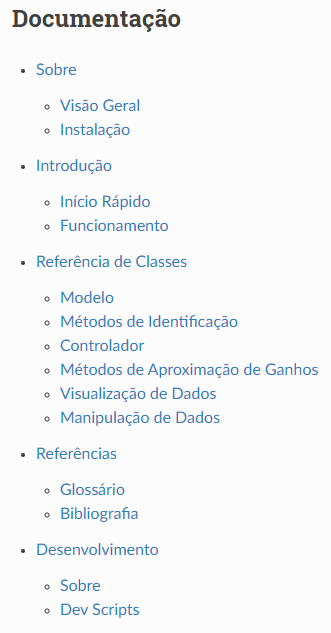
\includegraphics[scale=0.6]{figuras/doc_summary}
    \label{fig:doc_summary}
    \\
    \vspace{0cm}\hspace{0cm}\small{Fonte: Do autor}
\end{figure}

Cada uma das páginas desenvolvida abora um ponto importante sobre o projeto, da seguinte forma:
\begin{itemize}
    \item ``Sobre'': fornece uma breve descrição do projeto, seguida de uma explicação de como realizar a instalação da
    biblioteca;
    \item ``Introdução'': apresenta um guia rápido, ensinando e exemplificando de forma simples e prática o uso básico das
    funcionalidades, após isso é descrita uma visão estrutural do projeto;
    \item ``Referência de Classes'': Lista todas as classes implementadas, agrupando por função;
    \item ``Referências'': contempla o glossário e as referências utilizadas por toda a documentação;
    \item ``Desenvolvimento'': explora o desenvolvimento da biblioteca e traz breve listagem de scripts úteis para
    o desenvolvimento.
\end{itemize}


\section{Testes}

Foi realizado o desenvolvimento de testes para a maioria das funcionalidades da biblioteca, ajudando na detecção
rápida de novos bugs e facilitando futuras implementações.
Uma boa parte do código desenvolvido foi coberto por esses testes, como pode ser visto na figura \ref{fig:coverage}.

\begin{figure}[H]
    \centering
    \caption{Visualização do relatório de cobertura}
    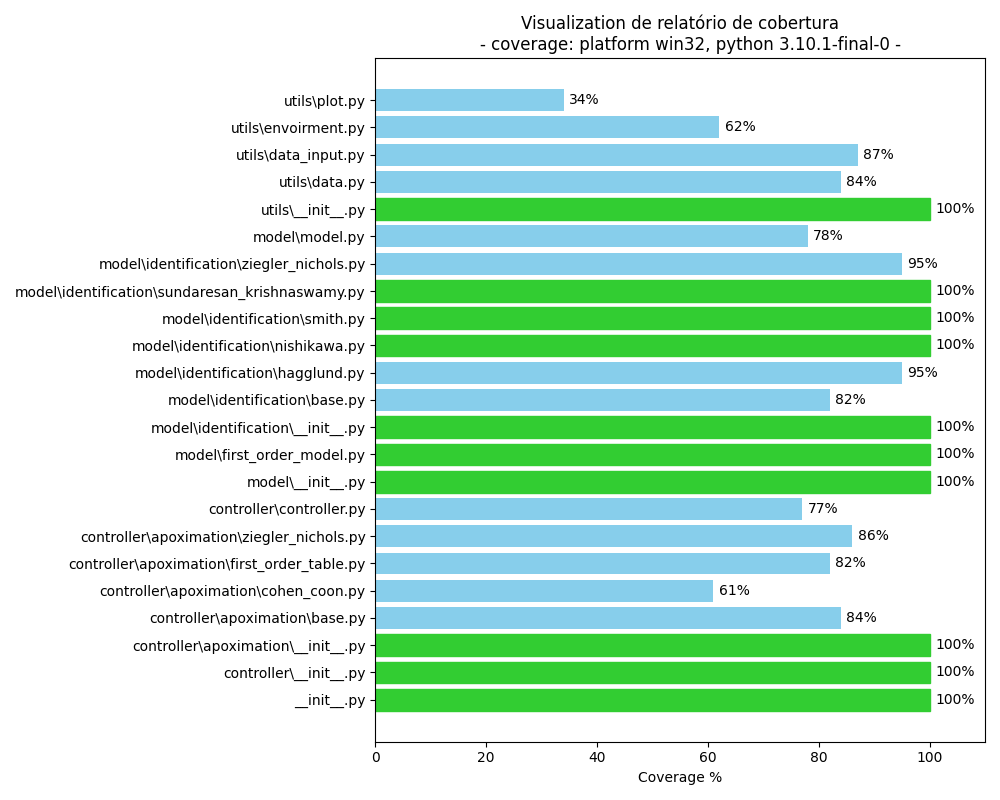
\includegraphics[scale=0.6]{figuras/coverage}
    \label{fig:coverage}
    \\
    \vspace{0cm}\hspace{0cm}\small{Fonte: Do autor}
\end{figure}


\section{Usabilidade}

A biblioteca foi projetada para um uso ágil e simples, de forma que com poucas linhas de código é possível realizar a
identificação de um modelo e a aproximação de ganhos de um controlador, bem como obter informações de suas respostas
a sinal degrau e gráficos para visualização.

Para um caso onde se deseja identificar o modelo de uma planta através do método de Nishikawa e obter um controlador
pelo método de Cohen e Coon, o primeiro paço é importar a biblioteca e obter o leiaute para entrada dos dados:

\begin{lstlisting}[label={lst:get_dil}]
import auto_control_tools as act

act.NishikawaModelIdentification.get_data_input_layout('./', save_as='csv', no_sample_time=True)
\end{lstlisting}

Com isso um arquivo \("\)data\_input.csv\("\) será criado no diretório atual.
Os dados de resposta do sistema devem ser inseridos nele, nesse caso no formato CSV, com os dados separados por vírgula.
O parâmetro no\_sample\_time foi marcado como verdadeiro, indicando para o método de criação do leiaute que não
se deseja informar os dados de tempo de aquisição na planilha fornecida.
Esse dado pode ser fornecido posteriormente como uma constante.

Com o arquivo preenchido com os dados de resposta a sinal degrau do sistema, é possível realizar a identificação,
obtendo um modelo em que é possível visualizar os dados e o gráfico de forma simples, como pode ser visto no trecho
de código a seguir:

\begin{lstlisting}[label={lst:get_model}]
import auto_control_tools as act

# act.NishikawaModelIdentification.get_data_input_layout('./', save_as='csv', no_sample_time=True)

model = act.NishikawaModelIdentification.get_model('./data_input.csv', sample_time=1, ignore_delay_threshold=0)

model.view.print_tf()
model.view.print_model_step_response_data()
model.view.plot_model_step_response_graph()
\end{lstlisting}

Para os dados fornecidos, a execução do código imprime as seguintes informações no terminal:
\begin{lstlisting}[label={lst:get_model_out}]
0.841304347826087*exp(-2.22428940568476*s)/(7.60658914728682*s + 1.0)
{'Overshoot': 0,
 'Peak': 0.841304292382592,
 'PeakTime': 128.0,
 'RiseTime': 16.726793943383804,
 'SettlingMax': 0.8413043478260871,
 'SettlingMin': 0.7574087299857988,
 'SettlingTime': 32.02106649111257,
 'SteadyStateValue': 0.8413043478260871,
 'Undershoot': 0.6269523372311043}
\end{lstlisting}

Além disso é aberta uma janela interativa, onde pode ser comparado o resultado da identificação com os dados de entrada
como pode ser visto na figura \ref{fig:get_model_plot}, que apresenta a janela com a visualização dos dados discretos
com a resposta a sinal degrau do modelo gerado sobreposta, para fins de visualização da proximidade entre o modelo
gerado e os dados discretos inseridos.
Nesse caso a resposta do modelo está sendo redimensionada em relação ao valor do \textit{setpoint}, para ser possível a
comparação com os dados de entrada.

\begin{figure}[H]
    \centering
    \caption{Exemplo de uso da biblioteca - plot\_model\_step\_response\_graph}
    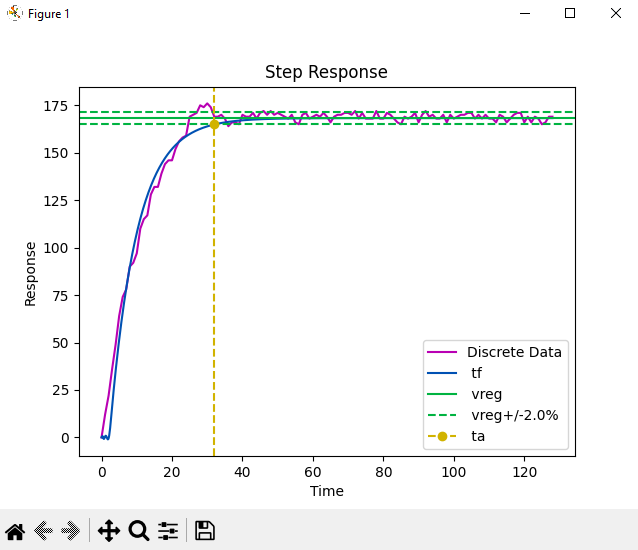
\includegraphics[scale=0.6]{figuras/get_model_plot}
    \label{fig:get_model_plot}
    \\
    \vspace{0cm}\hspace{0cm}\small{Fonte: Do autor}
\end{figure}

O processo de aproximação de ganhos de controlador por Cohen Coon ocorre de forma ainda mais simples, apenas é
necessário fornecer o modelo e o controlador desejado, a etapa de visualização de dados ocorre de forma
idêntica como pode ser visto no trecho de código a seguir:

\begin{lstlisting}[label={lst:get_controller}]
controller = act.CohenCoonControllerAproximation.get_controller(model, act.PID)

controller.view.print_tf()
controller.view.print_controller_step_response_data()
controller.view.plot_controller_step_response_graph()
\end{lstlisting}

Como pode ser visto na sequência, a execução produz uma saida idêntica no terminal, mas agora para o sistema em malha
fechada com o controlador gerado:

\begin{lstlisting}[label={lst:get_controller_out}]
0.841304347826087*(0.768000555728862*s + 5.71697021219369 + 4.89459279701174/s)*exp(-2.22428940568476*s)/((1 + 0.841304347826087*(0.768000555728862*s + 5.71697021219369 + 4.89459279701174/s)*exp(-2.22428940568476*s)/(7.60658914728682*s + 1.0))*(7.60658914728682*s + 1.0))
{'Kd': 0.7680005557288616,
 'Ki': 4.89459279701174,
 'Kp': 5.716970212193688,
 'Overshoot': 22.98302475453806,
 'Peak': 1.2298302475453806,
 'PeakTime': 5.9407504937458855,
 'RiseTime': 1.6853192890059248,
 'SettlingMax': 1.2298302475453806,
 'SettlingMin': 0.9145088850141698,
 'SettlingTime': 12.850559578670177,
 'SteadyStateValue': 1.0,
 'Undershoot': 7.829211261071754}
\end{lstlisting}

O gráfico de resposta plotado por padrão também traz a resposta do modelo em malha aberta para comparação.
Esse comportamento pode ser alterado informando o parâmetro plot\_model como False.
O resultado da plotagem pode ser visto na figura \ref{fig:get_controller_plot}, em que é apresentada a resposta a sinal
degrau unitário do modelo em comparação a resposta a um \textit{setpoint} unitário da planta em malha fechada,
possibilitando assim tanto a comparação da do caso de malha aberta com o caso de malha fechada, quanto a observação
gráfica do desempenho do controlador.

\begin{figure}[H]
    \centering
    \caption{Exemplo de uso da biblioteca - plot\_controller\_step\_response\_graph}
    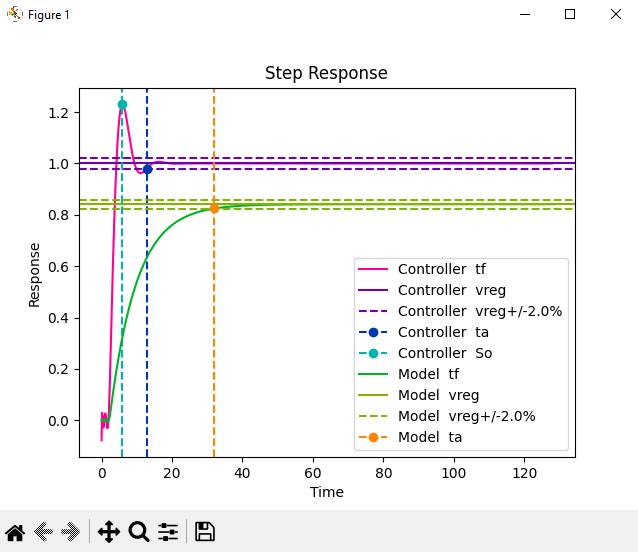
\includegraphics[scale=0.6]{figuras/get_controller_plot}
    \label{fig:get_controller_plot}
    \\
    \vspace{0cm}\hspace{0cm}\small{Fonte: Do autor}
\end{figure}

Adicionalmente, a janela interativa suporta ampliar o gráfico, para melhor visualização da resposta do sistema em
malha fechada, por exemplo.
Uma vista ampliada pode ser observada na figura \ref{fig:get_controller_plot_zoom}.

\begin{figure}[H]
    \centering
    \caption{Exemplo de uso da biblioteca - plot\_controller\_step\_response\_graph - Zoom}
    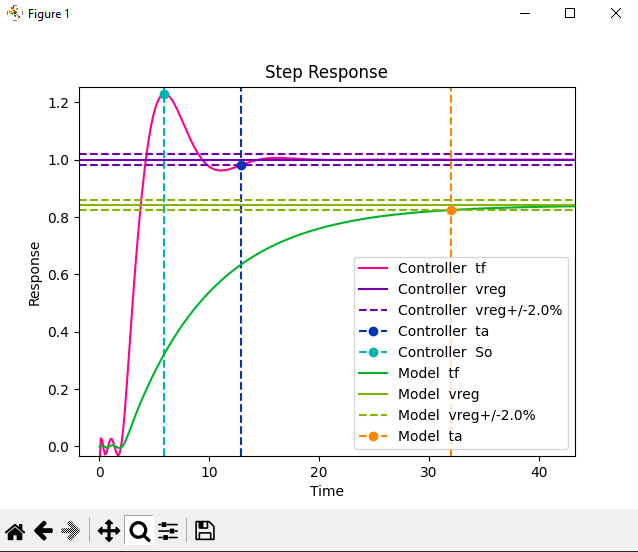
\includegraphics[scale=0.6]{figuras/get_controller_plot_zoom}
    \label{fig:get_controller_plot_zoom}
    \\
    \vspace{0cm}\hspace{0cm}\small{Fonte: Do autor}
\end{figure}

As mesmas operações podem ser executadas em qualquer ambiente com uma versão de Python suportada, inclusive em
ambientes Jupyter.
A seguir, é demonstrada a execução do mesmo código do exemplo anterior, mas desta vez no Google Colab,
um serviço gratuito da empresa Google que permite escrever e executar código Python através do navegador em um ambiente
baseado em Jupyter.
Além de estar sendo executado em nuvem, o ambiente baseado em Jupyter possibilita uma formatação mais visualmente
agradável das funções de transferência e das informações de resposta a sinal degrau.

Na figura \ref{fig:colab_example1}, são apresentadas duas células de execução, a primeira fazendo a instalação da
biblioteca utilizando pip, e a segunda importando a biblioteca e também é obtido o modelo de input de dados para
o método de identificação a ser utilizado.

\begin{figure}[H]
    \centering
    \caption{Exemplo de uso da biblioteca - execução no colab - instalação importação e obtenção de leiaute}
    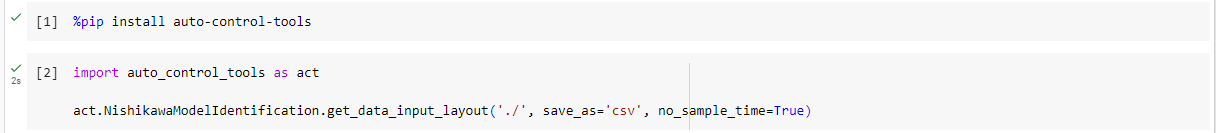
\includegraphics[scale=0.5]{figuras/colab_example1}
    \label{fig:colab_example1}
    \\
    \vspace{0cm}\hspace{0cm}\small{Fonte: Do autor}
\end{figure}

Em seguida, na figura \ref{fig:colab_example2} é realizado o processo de identificação pelo método de Nishikawa,
além de serem apresentados a função de transferência referente ao modelo obtido, os dados referentes a resposta do
modelo a sinal degrau, e o mesmo gráfico apresentado na figura \ref{fig:get_model_plot}.

\begin{figure}[H]
    \centering
    \caption{Exemplo de uso da biblioteca - execução no colab - obtenção e visualização de modelo}
    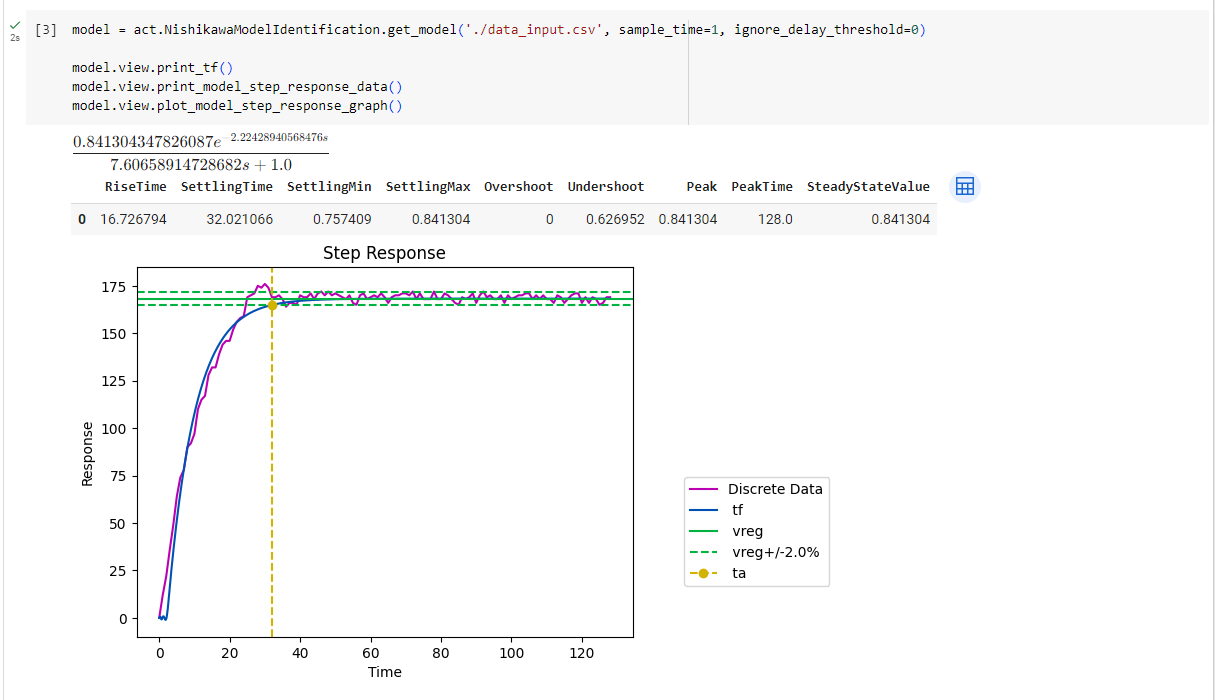
\includegraphics[scale=0.5]{figuras/colab_example2}
    \label{fig:colab_example2}
    \\
    \vspace{0cm}\hspace{0cm}\small{Fonte: Do autor}
\end{figure}

Por fim, é apresentada na figura \ref{fig:colab_example3} a célula com o código referente ao processo de aproximação de
ganhos de controlador PID pelo método C-C, além de serem apresentados a função de transferência referente ao sistema em
malha fechada, os dados referentes a resposta do sistema em malha fechada a um \textit{setpoint} unitário, e o mesmo
gráfico apresentado na figura \ref{fig:get_controller_plot}.

\begin{figure}[H]
    \centering
    \caption{Exemplo de uso da biblioteca - execução no colab - obtenção e visualização de controlador}
    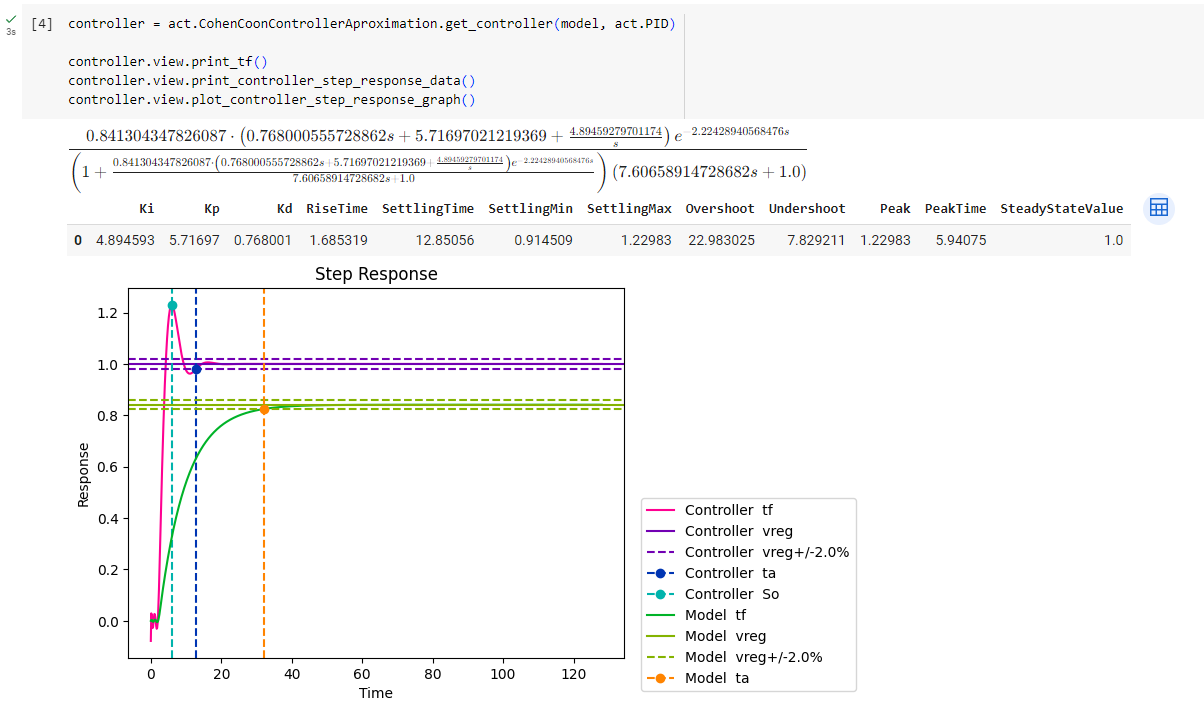
\includegraphics[scale=0.5]{figuras/colab_example3}
    \label{fig:colab_example3}
    \\
    \vspace{0cm}\hspace{0cm}\small{Fonte: Do autor}
\end{figure}


\section{Comparação com a Bibliografia}

As bibliografias de \cite{ogata2010engenharia} e \cite{CoelhoIdentificacao}, apesar de tratarem de identificação de
modelos, não fornecem dados discretos de resposta a sinal degram para poderem ser comparados aos métodos de
identificação implementados, desta forma esta seção de comparação com a bibliografia tratará apenas dos métodos de
aproximação de ganhos de controladores PID implementados.

\subsection{Biblioteca versus Apostila sobre PID e Métodos de Sintonia}

Para validarmos os resultados obtidos, podemos usar o exemplo do tanque aquecido de \cite{apostpidsint}.
Nele é apresentado o gráfico da figura \ref{fig:bib_comp_1_graph} e determinados os parâmetros $K$, $\tau$ e $\theta$ para
obtenção do modelo clássico que a classe FirstOrderModel da seção \ref{subsubsec:fom} se especializa.
Os valores calculados podem ser vistos em \ref{eq:bib_comp_1_id} e o modelo obtido é apresentado em
\ref{eq:bib_comp_1_model}.
E os resultados da aproximação de ganhos de controlador obtidos são descritos na tabela \ref{tab:bib_comp_1_restb}.


\begin{figure}[H]
    \centering
    \caption{Curva de reação para o tanque aquecido}
    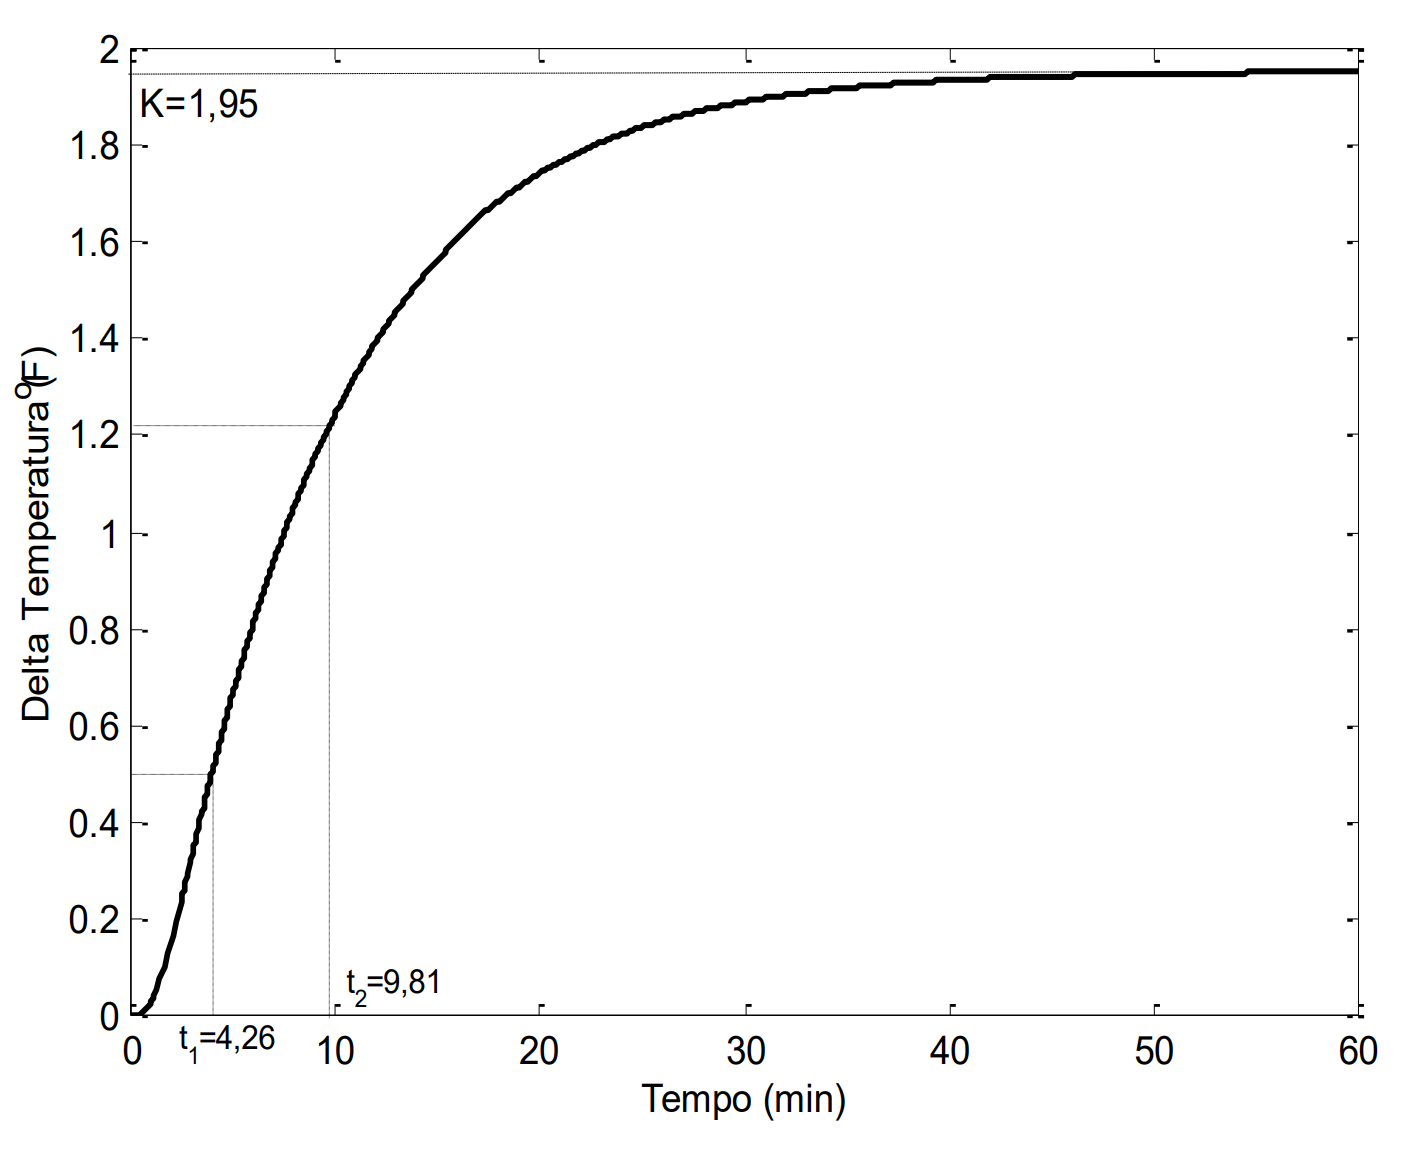
\includegraphics[scale=0.4]{figuras/bib_comp_1_graph}
    \label{fig:bib_comp_1_graph}
    \\
    \vspace{0cm}\hspace{0cm}\small{Fonte: \cite{apostpidsint}}
\end{figure}

\begin{equation}
    \label{eq:bib_comp_1_id}
    \tau = \frac{3}{2}(t_2 - t_1) = 8,33min \;\;,\;\; \theta = t_2 - T = 1,48min \;\;,\;\; K=1,95
\end{equation}

\begin{equation}
    \label{eq:bib_comp_1_model}
    G(s) = \frac{1,95}{8.33 s + 1}e^{-1,48 s}
\end{equation}

\begin{table}[h]
    \begin{center}
        \begin{tabular}{ | l | c | c | c | }
            \hline
            {}                         & {$K_P$} & {$T_I$}   & {$T_D$}   \\
            \hline
            {\textbf{Ziegler-Nichols}} & {3,46}  & {2,96min} & {0,74min} \\
            \hline
            {\textbf{Cohen-Coon}}      & {3,97}  & {3,39min} & {0,52min} \\
            \hline
        \end{tabular}
        \caption{ Métodos da curva de reação para o tanque aquecido}
        \vspace{0cm}\hspace{0cm}\small{Fonte: \cite{apostpidsint}}
        \label{tab:bib_comp_1_restb}
    \end{center}
\end{table}

Para comparação, pode-se instanciar um objeto de modelo com FirstOrderModel, utilizando os mesmos parâmetros fornecidos,
e então utilizar os métodos de aproximação de Ziegler e Nichols e de Cohen e Coon, como é disposto no trecho de código
a seguir:
\begin{lstlisting}[label={lst:bib_comp_1_code1}]
import auto_control_tools as act

model = act.FirstOrderModel(K=1.95, tau=8.33, theta=1.48)

model.view.print_tf()
model.view.print_model_step_response_data()
model.view.plot_model_step_response_graph()

controller = act.ZieglerNicholsControllerAproximation.get_controller(model, act.PID)

controller.view.print_tf()
controller.view.print_controller_step_response_data()
controller.view.plot_controller_step_response_graph()

controller = act.CohenCoonControllerAproximation.get_controller(model, act.PID)

controller.view.print_tf()
controller.view.print_controller_step_response_data()
controller.view.plot_controller_step_response_graph()
\end{lstlisting}

A execução de \ref{lst:bib_comp_1_code1} gera o resultado apresentado em \ref{lst:bib_comp_1_code1_out}
e os gráficos das figuras \ref{fig:bib_comp_1_code1_out_fig1}, \ref{fig:bib_comp_1_code1_out_fig2} e
\ref{fig:bib_comp_1_code1_out_fig3}.

\begin{lstlisting}[label={lst:bib_comp_1_code1_out}]
1.95*exp(-1.48*s)/(8.33*s + 1.0)
{'Overshoot': 0,
 'Peak': 1.9476708568782817,
 'PeakTime': 57.541601473921176,
 'RiseTime': 18.302321365061147,
 'SettlingMax': 1.95,
 'SettlingMin': 1.755565040374366,
 'SettlingTime': 34.082117580267,
 'SteadyStateValue': 1.95,
 'Undershoot': 0.38160197607648316}
1.95*(2.56307692307692*s + 3.46361746361746 + 1.1701410350059/s)*exp(-1.48*s)/((1 + 1.95*(2.56307692307692*s + 3.46361746361746 + 1.1701410350059/s)*exp(-1.48*s)/(8.33*s + 1.0))*(8.33*s + 1.0))
{'Kd': 2.563076923076923,
 'Ki': 1.1701410350058998,
 'Kp': 3.4636174636174637,
 'Overshoot': 8.369513829384001,
 'Peak': 1.08369513829384,
 'PeakTime': 7.7288758064631535,
 'RiseTime': 3.948447422867046,
 'SettlingMax': 1.08369513829384,
 'SettlingMin': 0.900405905739516,
 'SettlingTime': 12.825453331014943,
 'SteadyStateValue': 1.0,
 'Undershoot': 37.50000000000001}
1.95*(2.07319868112764*s + 3.97666897666898 + 1.17187743876933/s)*exp(-1.48*s)/((1 + 1.95*(2.07319868112764*s + 3.97666897666898 + 1.17187743876933/s)*exp(-1.48*s)/(8.33*s + 1.0))*(8.33*s + 1.0))
{'Kd': 2.073198681127638,
 'Ki': 1.1718774387693307,
 'Kp': 3.9766689766689765,
 'Overshoot': 6.845750381802541,
 'Peak': 1.0684575038180253,
 'PeakTime': 7.255513442274729,
 'RiseTime': 3.725804200087023,
 'SettlingMax': 1.0684575038180253,
 'SettlingMin': 0.9034279684915225,
 'SettlingTime': 12.269941651414406,
 'SteadyStateValue': 0.9999999999999999,
 'Undershoot': 32.67455930152555}
\end{lstlisting}



\begin{figure}[H]
    \centering
    \caption{Comparação de resultados - Bibliografia 1 - Gráfico do modelo}
    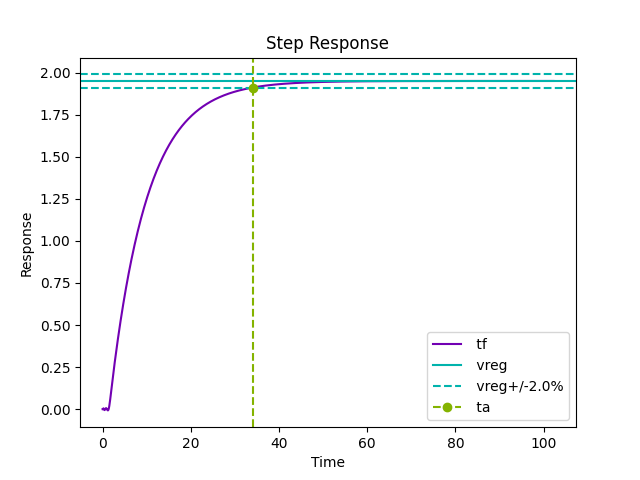
\includegraphics[scale=0.8]{figuras/bib_comp_1_code1_out_fig1}
    \label{fig:bib_comp_1_code1_out_fig1}
    \\
    \vspace{0cm}\hspace{0cm}\small{Fonte: Do autor}
\end{figure}
\begin{figure}[H]
    \centering
    \caption{Comparação de resultados - Bibliografia 1 - Gráfico Ziegler Nichols}
    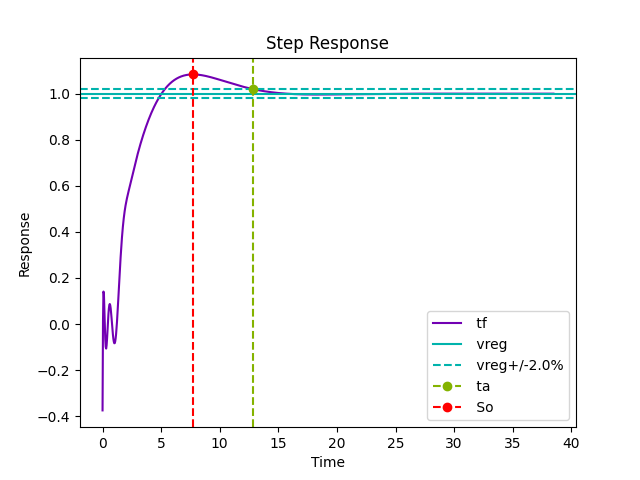
\includegraphics[scale=0.8]{figuras/bib_comp_1_code1_out_fig2}
    \label{fig:bib_comp_1_code1_out_fig2}
    \\
    \vspace{0cm}\hspace{0cm}\small{Fonte: Do autor}
\end{figure}
\begin{figure}[H]
    \centering
    \caption{Comparação de resultados - Bibliografia 1 - Gráfico Cohen Coon}
    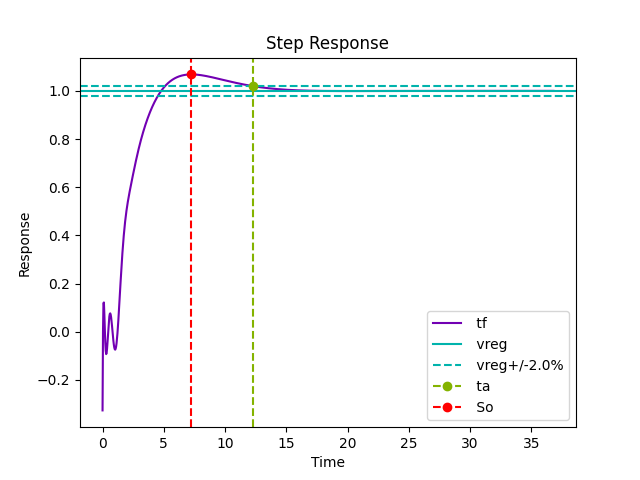
\includegraphics[scale=0.8]{figuras/bib_comp_1_code1_out_fig3}
    \label{fig:bib_comp_1_code1_out_fig3}
    \\
    \vspace{0cm}\hspace{0cm}\small{Fonte: Do autor}
\end{figure}

Calculando $T_I$ e $T_D$ de acordo com a equação \ref{eq:titd}, podemos verificar que os resultados das aproximações de
ganhos concordam com a bibliográfica, conforme detalha a tabela \ref{tab:bib_comp_1_pid_comp}.

\begin{equation}
    \label{eq:titd}
    Ki = \frac{Kp}{Ti} \;\; , \;\; Kd = Kp \times Td
\end{equation}

\begin{table}[h]
    \begin{center}
        \begin{tabular}{ | l | c | c | c | }
            \hline
            {}                                    & {$K_P$}              & {$T_I$}         & {$T_D$}         \\
            \hline
            {\textbf{Ziegler-Nichols}}            & {3,46}               & {2,96min}       & {0,74min}       \\
            \hline
            {\textbf{Cohen-Coon}}                 & {3,97}               & {3,39min}       & {0,52min}       \\
            \hline
            {\textbf{Ziegler-Nichols Biblioteca}} & {3.4636174636174637} & {2,96}          & {0,74}          \\
            \hline
            {\textbf{Cohen-Coon Biblioteca}}      & {3.9766689766689765} & {3.39341713144} & {0.52134052225} \\
            \hline
        \end{tabular}
        \caption{ Métodos da curva de reação para o tanque aquecido}
        \vspace{0cm}\hspace{0cm}\small{Fonte: Do autor}
        \label{tab:bib_comp_1_pid_comp}
    \end{center}
\end{table}

Contudo, ao comparar os gráficos \ref{fig:bib_comp_1_code1_out_fig2} e \ref{fig:bib_comp_1_code1_out_fig3} com as
respostas apresentadas na figura \ref{fig:bib_comp_1_ctrl_fig},
nota-se uma ligeira diferença no sobressinal entre o gráfico da biblioteca e da bibliografia.
Foram feitos testes em outros sistemas, tentando reproduzir o resultado da bibliografia, contudo apenas resultados
idênticos ao apresentado pela biblioteca foram observados.

\begin{figure}[H]
    \centering
    \caption{Comparação de resultados - Bibliografia 1 - Gráfico Cohen Coon}
    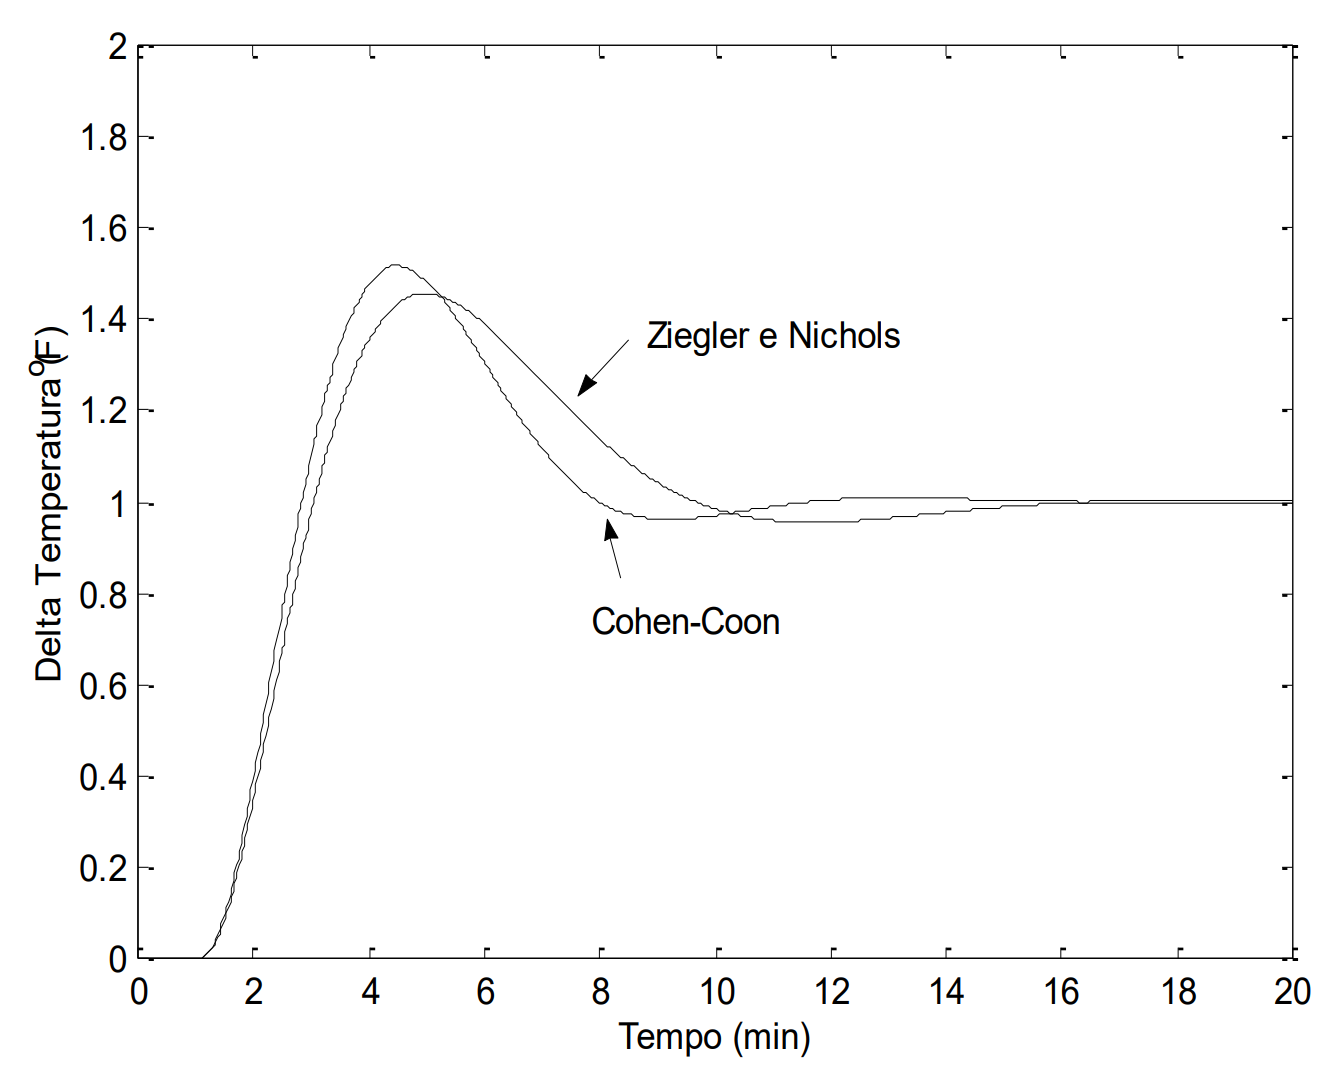
\includegraphics[scale=0.4]{figuras/bib_comp_1_ctrl_fig}
    \label{fig:bib_comp_1_ctrl_fig}
    \\
    \vspace{0cm}\hspace{0cm}\small{Fonte: Do autor}
\end{figure}


\section{Comaprações com Experimentos Anteriores}

Afim demonstrar a capacidade da biblioteca de realizar identificações e aproximações de
controlador de forma rápida e em massa, foram pegos dados já existentes de resposta a sinal degrau de algumas plantas
didáticas do laboratório de controle do Campus do IFSC\@.
Optou-se por fazer o processo de identificação utilizando o método Smith e a aproximação de ganhos de controlador
com o método Cohen Coon.

As plantas trabalhadas são um forno, uma mesa giratória e o nível de um tanque.
Detalhes sobre variáveis manipulada e controlada foram abstraídos por não serem o foco da comparação.
As plantas trabalhadas, em geral, possuíam resposta rápida, com atraso baixo ou nulo, o que, em alguns casos,
impossibilitou o uso do método de Cohen e Coon.
Os resultados das identificações e controladores podem ser observados
nas tabelas \ref{tab:results_forno}, \ref{tab:results_mesa}, \ref{tab:results_tanque}.

\begin{table}[H]
    \caption{Resultados obtidos - Forno}
    \centering
    \begin{tabular}{|c|c|c|c|c|c|c|}
        \hline
        \textbf{Setpoint} & \textbf{Modelo}                          & \textbf{Kp} & \textbf{Ki} & \textbf{Kd} & \textbf{Identificação} & \textbf{Malha fechada} \\
        \hline
        15\%              & $\frac{18.08 e^{-22.5s}}{1144.5s + 1.0}$ & 3.76        & 0.068       & 30.70       & 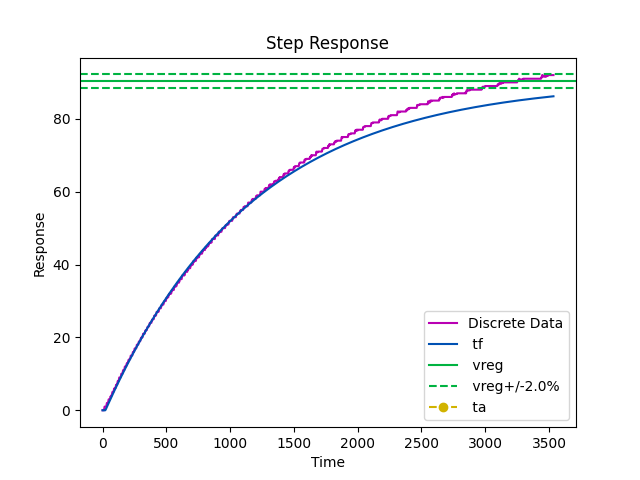
\includegraphics[width=0.2\linewidth]{figuras/forno_15} & 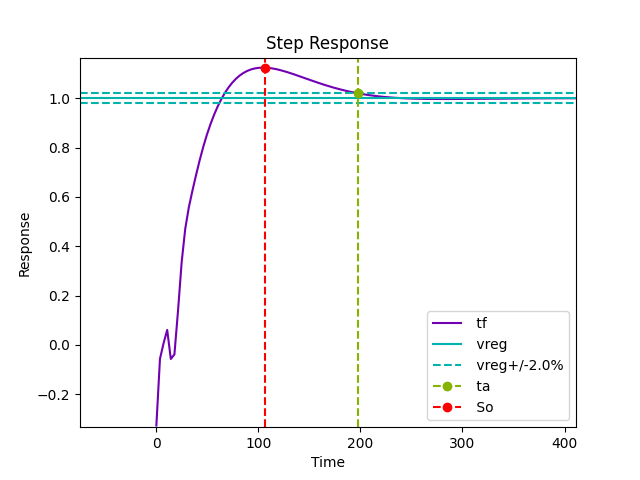
\includegraphics[width=0.2\linewidth]{figuras/forno_15c} \\
        \hline
        20\%              & $\frac{6.90 e^{-19.5s}}{919.5s + 1.0}$   & 9.14        & 0.192       & 64.57       & 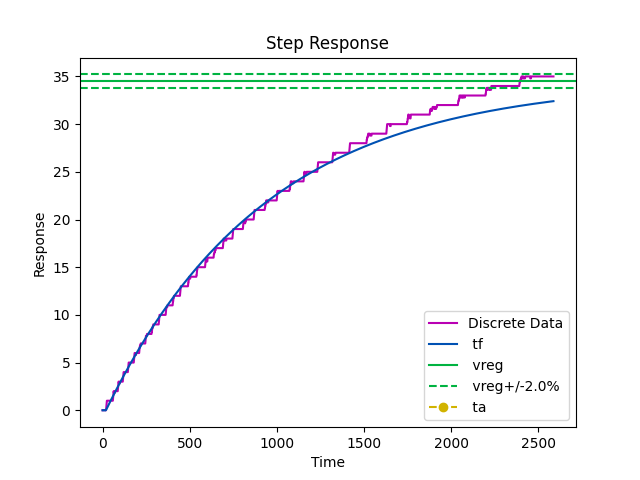
\includegraphics[width=0.2\linewidth]{figuras/forno_20} & 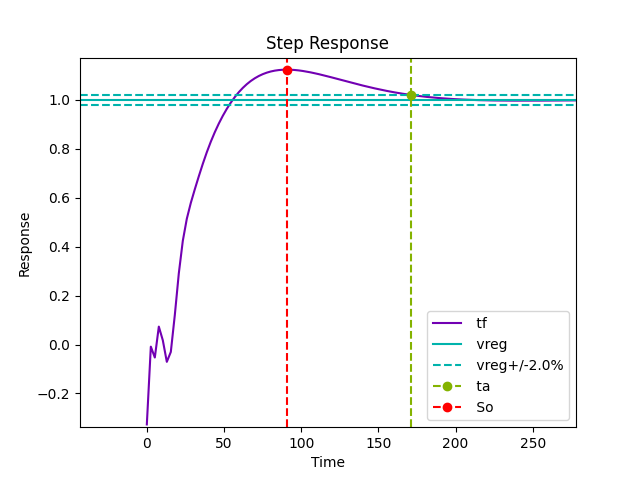
\includegraphics[width=0.2\linewidth]{figuras/forno_20c} \\
        \hline
        25\%              & $\frac{6.68 e^{-17.5s}}{997.5s + 1.0}$   & 11.42       & 0.267       & 72.41       & 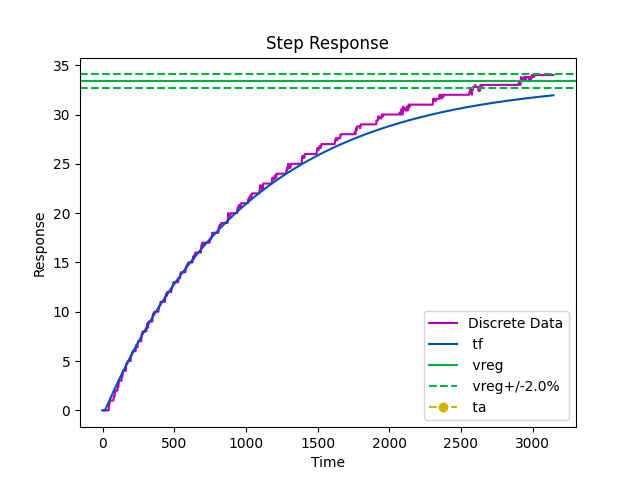
\includegraphics[width=0.2\linewidth]{figuras/forno_25} & 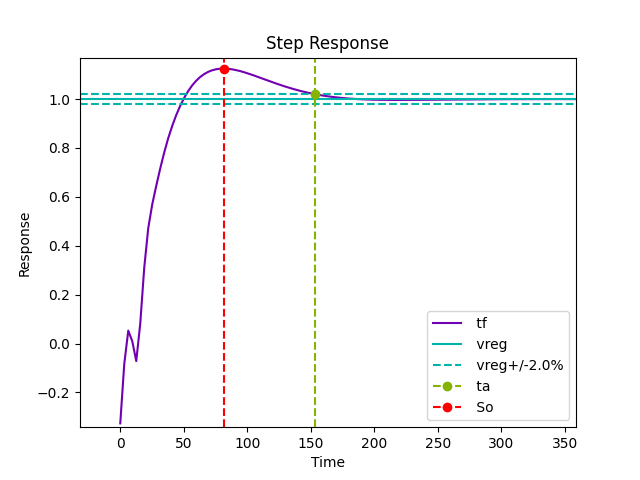
\includegraphics[width=0.2\linewidth]{figuras/forno_25c} \\
        \hline
    \end{tabular}
    \label{tab:results_forno}
    \vspace{0cm}\hspace{0cm}\small{Fonte: Do autor}
\end{table}


\begin{table}[H]
    \caption{Resultados obtidos - Mesa Giratória}
    \centering
    \begin{tabular}{|c|c|c|c|c|c|c|}
        \hline
        \textbf{Setpoint} & \textbf{Modelo}                       & \textbf{Kp} & \textbf{Ki} & \textbf{Kd} & \textbf{Identificação} & \textbf{Malha fechada} \\
        \hline
        Mesa (5-10\%)     & $\frac{25.93 e^{-1.5s}}{52.5s + 1.0}$ & 1.81        & 0.496       & 0.982       & 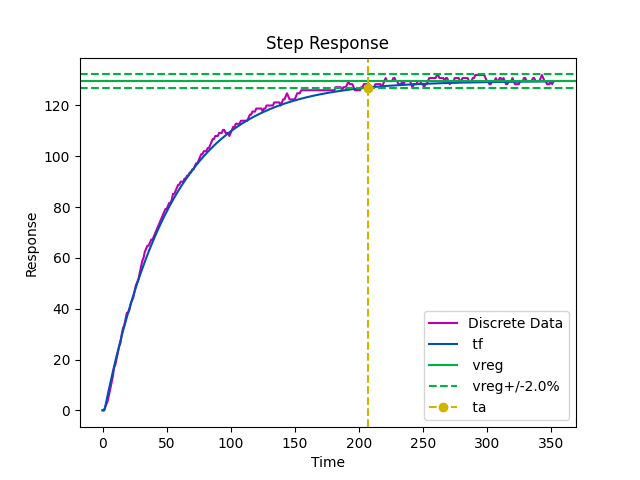
\includegraphics[width=0.2\linewidth]{figuras/mesa_5_10} & 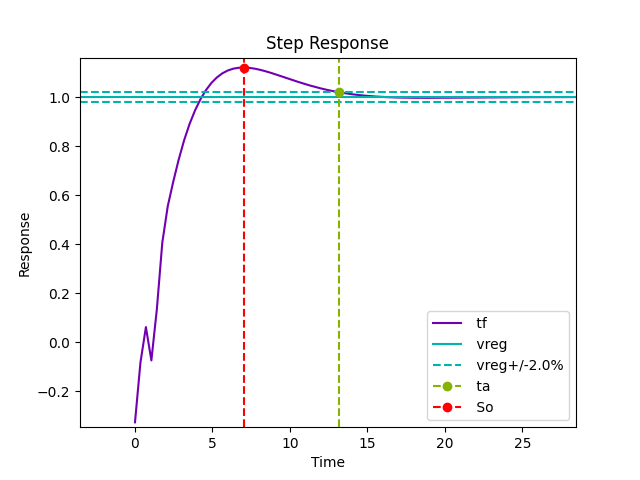
\includegraphics[width=0.2\linewidth]{figuras/mesa_5_10c} \\
        \hline
        Mesa (10-15\%)    & $\frac{17.81 e^{-3.5s}}{40.5s + 1.0}$ & 0.88        & 0.106       & 1.10        & 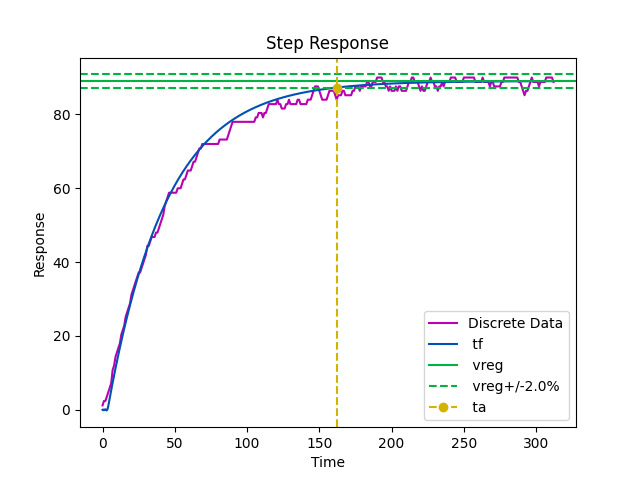
\includegraphics[width=0.2\linewidth]{figuras/mesa_10_15} & 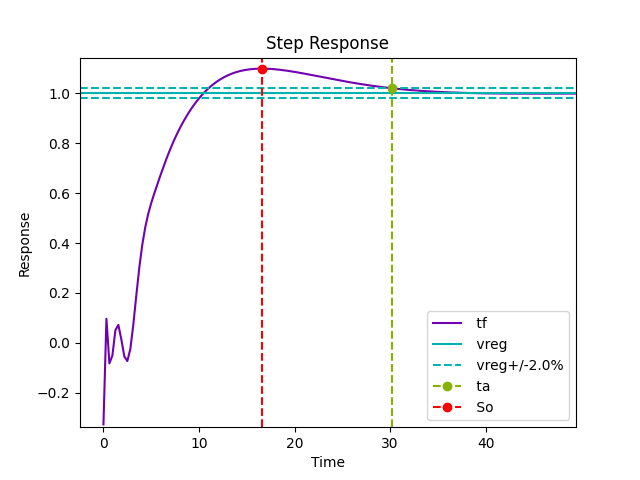
\includegraphics[width=0.2\linewidth]{figuras/mesa_10_15c} \\
        \hline
        Mesa (15-17\%)    & $\frac{15.3}{54.0s + 1.0}$            & -           & -           & -           & 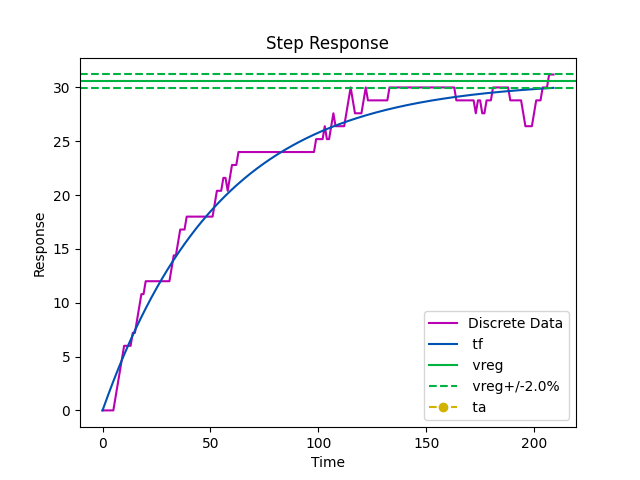
\includegraphics[width=0.2\linewidth]{figuras/mesa_15_17} & \textbf{Sem Atraso} \\
        \hline
        Mesa (17-20\%)    & $\frac{12.0}{37.5s + 1.0}$            & -           & -           & -           & 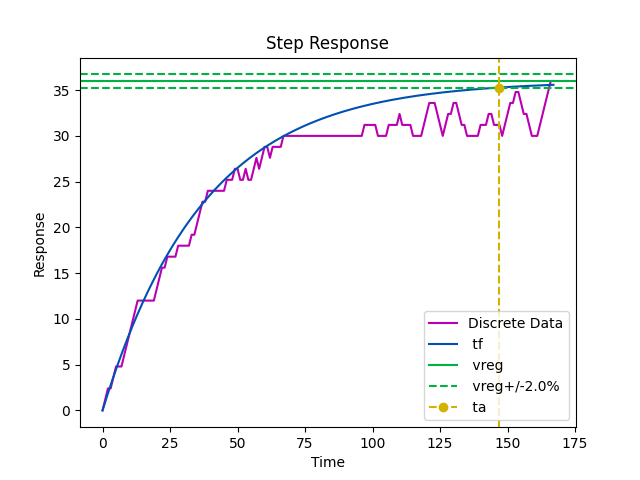
\includegraphics[width=0.2\linewidth]{figuras/mesa_17_20} & \textbf{Sem Atraso} \\
        \hline
    \end{tabular}
    \label{tab:results_mesa}
    \vspace{0cm}\hspace{0cm}\small{Fonte: Do autor}
\end{table}


\begin{table}[H]
    \caption{Resultados obtidos - Nível Tanque}
    \centering
    \begin{tabular}{|c|c|c|c|c|c|c|}
        \hline
        \textbf{Setpoint} & \textbf{Modelo}                      & \textbf{Kp} & \textbf{Ki} & \textbf{Kd} & \textbf{Identificação} & \textbf{Malha fechada} \\
        \hline
        Tanque (40-50\%)  & $\frac{2.58 e^{-2.0s}}{18.0s + 1.0}$ & 4.75        & 1.01        & 3.38        & 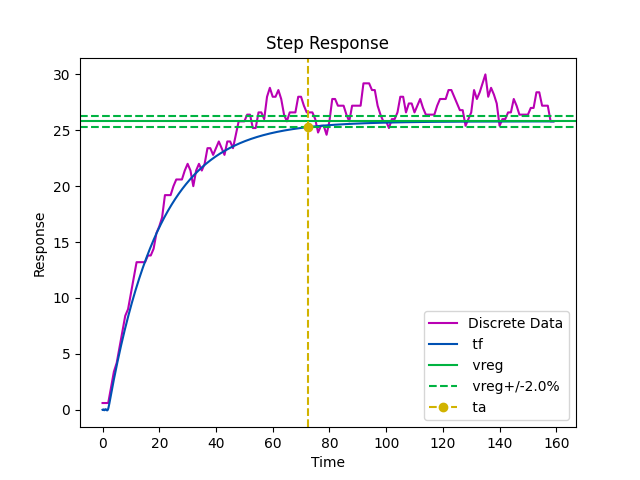
\includegraphics[width=0.2\linewidth]{figuras/tanque_40_50} & 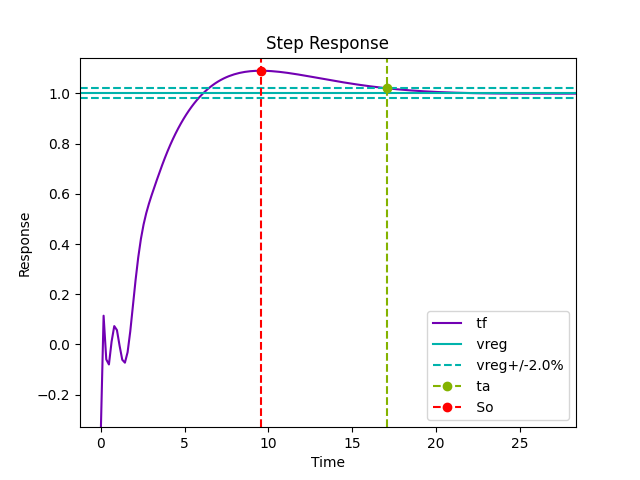
\includegraphics[width=0.2\linewidth]{figuras/tanque_40_50c} \\
        \hline
        Tanque (40-50\%)  & $\frac{3.77 e^{-1.0s}}{33.0s + 1.0}$ & 11.73       & 4.83        & 4.24        & 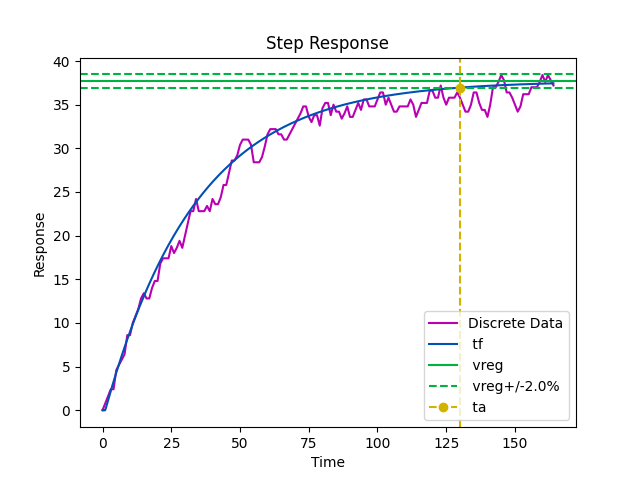
\includegraphics[width=0.2\linewidth]{figuras/tanque_50_60} & 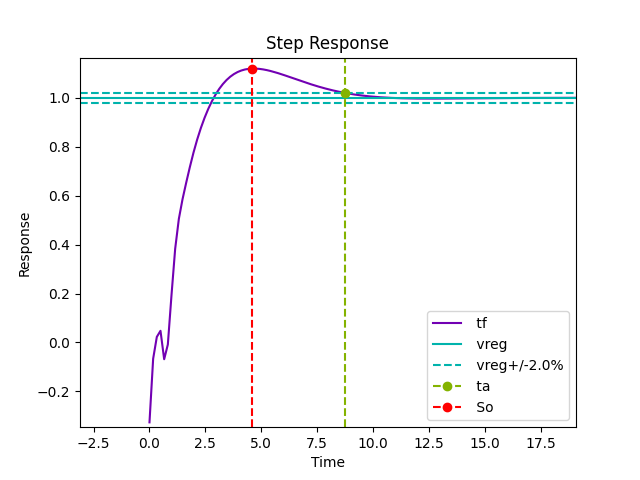
\includegraphics[width=0.2\linewidth]{figuras/tanque_50_60c} \\
        \hline
        Tanque (40-50\%)  & $\frac{3.45}{52.5s + 1.0}$           & -           & -           & -           & 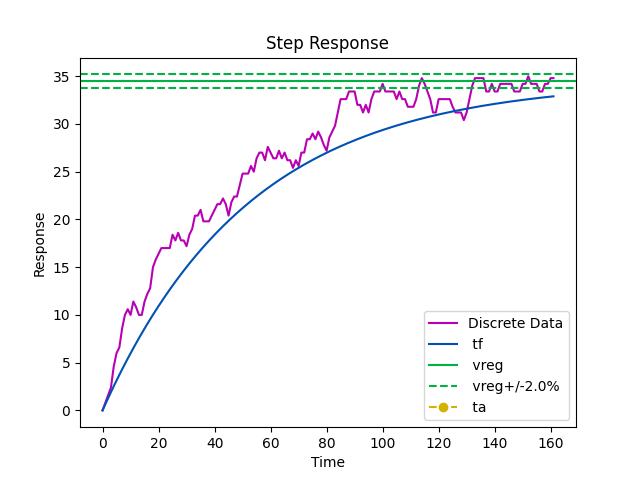
\includegraphics[width=0.2\linewidth]{figuras/tanque_60_70} & \textbf{Sem Atraso} \\
        \hline
        Tanque (40-50\%)  & $\frac{1.26 e^{-5.0s}}{6.0s + 1.0}$  & 1.47        & 0.156       & 2.32        & 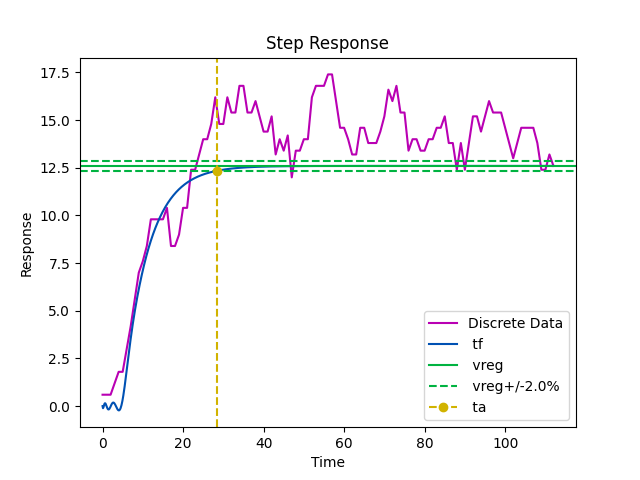
\includegraphics[width=0.2\linewidth]{figuras/tanque_70_80} & 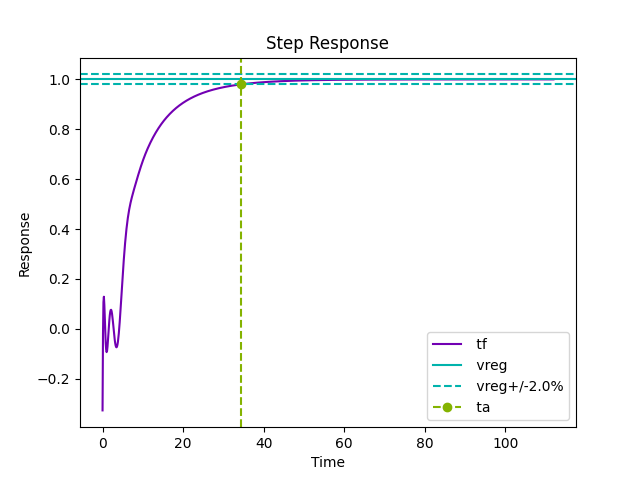
\includegraphics[width=0.2\linewidth]{figuras/tanque_70_80c} \\
        \hline
    \end{tabular}
    \label{tab:results_tanque}
    \vspace{0cm}\hspace{0cm}\small{Fonte: Do autor}
\end{table}

Para de validar os resultados obtidos, foram pegos também os modelos e os ganhos de controladores PID obtidos em um dos
trabalhos realizados para a planta Mesa Giratória.
Os modelos foram obtidos de forma manual com auxílio do mathlab através do método de identificação de Smith, os
resultados para as faixas de 5 a 10\%, de 10 a 15\%, de 15 a 17\% e de 17 a 20\% podem ser vistos nas equações
\ref{eq:comp_prev_eq1}, \ref{eq:comp_prev_eq2}, \ref{eq:comp_prev_eq3} e \ref{eq:comp_prev_eq4}, respectivamente.
Já os controladores, foram gerados através de ambos os métodos de aproximação de controlador PID Z-N e C-C, para os
casos de controlador P, PI e PID. Contudo, foram calculados apenas para a faixa de 10 a 15\%.
Os resultados obtidos para os ganhos de controlador podem ser observados nas tabelas
\ref{tab:comp_prev_zn} e \ref{tab:comp_prev_cc}.

\begin{equation}
    \label{eq:comp_prev_eq1}
    G(s) = \frac{27,6}{49,5 s + 1}e^{-0,5 s}
\end{equation}
\begin{equation}
    \label{eq:comp_prev_eq2}
    G(s) = \frac{18}{40,5 s + 1}e^{-3,5 s}
\end{equation}
\begin{equation}
    \label{eq:comp_prev_eq3}
    G(s) = \frac{18}{36 s + 1}e^{-2 s}
\end{equation}
\begin{equation}
    \label{eq:comp_prev_eq4}
    G(s) = \frac{12}{57 s + 1}e^{-4 s}
\end{equation}

\begin{table}[H]
    \caption{Resultados prévios - Controlador por Ziegler-Nichols}
    \centering
    \begin{tabular}{|l|l|l|l|}
        \hline
        \textbf{Type} & \textbf{$K_P$} & \textbf{$K_I$} & \textbf{$K_D$} \\
        \hline
        \textbf{P}    & 0.643          & -              & -              \\
        \hline
        \textbf{PI}   & 0.579          & 0.0496         & -              \\
        \hline
        \textbf{PID}  & 0.77           & 0.11           & 1.351          \\
        \hline
    \end{tabular}
    \label{tab:comp_prev_zn}
    \\
    \vspace{0cm}\hspace{0cm}\small{Fonte: Do autor}
\end{table}

\begin{table}[H]
    \caption{Resultados prévios - Controlador por Cohen-Coon}
    \centering
    \begin{tabular}{|l|l|l|l|}
        \hline
        \textbf{Type} & \textbf{$K_P$} & \textbf{$K_I$} & \textbf{$K_D$} \\
        \hline
        \textbf{P}    & 0.66           & -              & -              \\
        \hline
        \textbf{PI}   & 0.58           & 0.05876        & -              \\
        \hline
        \textbf{PID}  & 0.87           & 0.1047         & 1.088          \\
        \hline
    \end{tabular}
    \label{tab:comp_prev_cc}
    \\
    \vspace{0cm}\hspace{0cm}\small{Fonte: Do autor}
\end{table}

Modelos da planta Mesa Giratória utilizando os mesmos métodos já foram obtidos e apresentados na tabela
\ref{tab:results_mesa}.
Comparando os resultados, podemos observar que em geral foram obtidos modelos similares, com algumas divergências
provavelmente causadas pelos métodos utilizados para aferir o tempo de acomodação e por conseguinte os valores dos
momentos $t_1$ e $t_2$, com base na descrição do método em \ref{subsubsec:smfun}.

Para fins de comparação, foram gerados os ganhos PID através dos métodos Z-N e C-C para a mesma faixa dos resultados
anteriores, de 10 a 15\%, mas utilizando os controladores gerados pelo método de identificação de Smith da biblioteca
desenvolvida.
Os dados obtidos estão apresentados nas tabelas \ref{tab:comp_nw_zn} e \ref{tab:comp_nw_cc} para os métodos
Z-N e C-C respectivamente.


\begin{table}[H]
    \caption{Resultados novos - Controlador por Ziegler-Nichols}
    \centering
    \begin{tabular}{|l|l|l|l|}
        \hline
        \textbf{Type} & \textbf{kp} & \textbf{ki} & \textbf{kd} \\
        \hline
        P             & 0.6496      & -           & -           \\
        \hline
        PI            & 0.5846      & 0.0501      & -           \\
        \hline
        PID           & 0.7795      & 0.1114      & 1.3641      \\
        \hline
    \end{tabular}
    \label{tab:comp_nw_zn}
    \\
    \vspace{0cm}\hspace{0cm}\small{Fonte: Do autor}
\end{table}

\begin{table}[H]
    \caption{Resultados novos - Controlador por Cohen-Coon}
    \centering
    \begin{tabular}{|l|l|l|l|}
        \hline
        \textbf{Type} & \textbf{kp} & \textbf{ki} & \textbf{kd} \\
        \hline
        P             & 0.6496      & -           & -           \\
        \hline
        PI            & 0.5846      & 0.0501      & -           \\
        \hline
        PID           & 0.7795      & 0.1114      & 1.3641      \\
        \hline
    \end{tabular}
    \label{tab:comp_nw_cc}
    \\
    \vspace{0cm}\hspace{0cm}\small{Fonte: Do autor}
\end{table}


\section{Aplicação em Sistema Real}

Ainda não ocorreu

\chapter{Considerações Finais}

A evolução tecnológica na área de automação e controle de sistemas tem sido um fator determinante no avanço de inúmeras
indústrias e pesquisas científicas.
Ferramentas eficientes para a análise e controle de sistemas dinâmicos são essenciais não apenas para o desenvolvimento
de novas tecnologias, mas também para a otimização de processos existentes.
Em um contexto onde a precisão e a eficiência são cruciais, a necessidade de ferramentas capazes de simplificar e
agilizar estas tarefas torna-se evidente.
A habilidade de modelar e controlar sistemas de maneira eficiente tem implicações diretas na melhoria do desempenho,
segurança e qualidade em diversos setores.

Nesse cenário, este trabalho apresentou uma contribuição significativa ao desenvolver uma biblioteca em Python que
aborda a necessidade de ferramentas aprimoradas para análise e controle de sistemas dinâmicos.
Esta biblioteca, alinhada com as demandas do setor, combina eficácia e facilidade de uso, visando automatizar os
processos de identificação de modelo e aproximação de ganhos de controlador PID para sistemas de controle.
Compatível com diversos ambientes operacionais, a solução desenvolvida é acessível e valiosa tanto para profissionais
da área quanto para estudantes e pesquisadores.
A geral do trabalho de contribuir para um segmento crucial, atendendo às necessidades práticas e educacionais no
campo de automação e controle, foi efetivamente alcançado, destacando-se como um recurso inclusivo e acessível para a
comunidade.

A arquitetura escolhida para a biblioteca, enfatizando a compreensibilidade e a escalabilidade, garante não apenas a
eficácia imediata da ferramenta, mas também a facilidade de expansão futura.
A integração bem-sucedida com a biblioteca de controle para Python existente amplia as possibilidades de uso dos modelos
criados, proporcionando uma versatilidade notável à ferramenta.
Esta característica sublinha a capacidade da biblioteca de se adaptar e ser aplicável em uma variedade de cenários de
controle de sistemas.

Um aspecto fundamental deste trabalho é a concentração na usabilidade da biblioteca, especialmente considerando usuários
com conhecimento limitado em programação Python.
O design da ferramenta, orientado para a facilidade de uso, a torna acessível e prática, oferecendo uma ponte entre o
conhecimento teórico e a aplicação prática no campo de controle e automação.

Os métodos desenvolvidos para a identificação de modelos são intuitivos e requerem um mínimo de intervenção do usuário,
o que simplifica o processo de modelagem.
Além disso, as funções implementadas para a determinação automática ou simplificada de ganhos de controle PID
destacam-se pela sua eficiência, baseando-se nos modelos da planta e nas metas de desempenho do sistema.
Essas características demonstram a praticidade e a aplicabilidade da biblioteca em um contexto real.

A documentação clara e acessível da biblioteca é uma de suas maiores forças.
Não só facilita o uso da ferramenta, mas também serve como um recurso educativo importante, potencializando o impacto da biblioteca tanto no ensino quanto, na prática de controle de sistemas.
Assim, este trabalho não apenas atende às necessidades técnicas dos profissionais da área, mas também contribui
significativamente para a formação e o desenvolvimento de futuros profissionais e pesquisadores em automação e controle.

\section{Sugestões para trabalhos futuros}

Desde a fase inicial de concepção, incluindo o levantamento dos objetivos e o projeto, a biblioteca desenvolvida neste
trabalho foi concebida com a visão de um projeto de CI/CD.
Essa abordagem estratégica visou estabelecer uma base sólida com funcionalidades essenciais, criando um ambiente
propício não apenas para atender às necessidades simples, mas também para facilitar o desenvolvimento de soluções
futuras.
Esse entendimento claro da necessidade de expansibilidade e adaptabilidade foi considerado durante todo o
desenvolvimento do projeto.
Consequentemente, as sugestões para trabalhos futuros, apresentadas nesta seção, são um componente muito importante
do processo de desenvolvimento desde o início.
As sugestões apresentadas representam possibilidades de melhoria factíveis e com vantagens claras.

\subsection{Integração com ferramentas da biblioteca de controle}
A biblioteca de sistemas de controle dispõe de algumas ferramentas para projeto de controlador, nenhuma das quais foi
abordada pela biblioteca desenvolvida neste trabalho.
Visto que os modelos gerados pela biblioteca desenvolvida possuem o objeto principal de análise, a função de
transferência do modelo, e este objeto pertence à biblioteca de controle o uso dessas ferramentas para projeto de
controlador de já é possível.
Contudo, isso depende de um conhecimento mais aprofundado tanto da biblioteca desenvolvida quanto da biblioteca de
controle, e possivelmente conhecimentos em programação com Python.
A integração dessas ferramentas em novas classes de aproximação de controlador pode proporcionar o uso facilitado destas
ferramentas.

As seguintes funções da biblioteca de controle foram consideradas boas opções de integração:
\begin{itemize}
    \item \textbf{place}: esta função pode ser utilizada para alocação de polos do sistema em lugares específicos do plano $s$.
    \item \textbf{lqr}: possibilita o projeto de controladores do tipo Linear-Quadrático Regulador.
    Contudo, envolveria a implementação de um novo objeto de controlador, visto que atualmente apenas controladores PID
    são suportados;
    \item \textbf{sisotool}: por fim, a ferramenta sistool proporciona um ambiente interativo para aplicação do método
    de lugar das raízes;
    A própria biblioteca de controle disponibiliza a função rootlocus\_pid\_designer que tenta possibilitar o projeto
    de controlador PID de forma interativa utilizando a função sisotool por trás dos panos.
\end{itemize}


\subsection{Especialização para casos de ordens mais altas}
Os métodos de identificação implementados neste trabalho se especializam apenas no caso de sistemas de primeira ordem
com atraso, que entregam um objeto de modelo do sistema igualmente especializado.
Para facilitar a implementação de métodos de identificação de modelo e possivelmente de aproximação de ganhos de
controlador PID para sistemas de ordens mais altas, a criação de uma classe especializada em casos clássicos de
segunda ordem, por exemplo, é um passo crucial, que deve ser feito antes de qualquer método que trate de sistemas
de ordens mais altas especializados nesses casos clássicos.

\subsection{Outros métodos de identificação de modelo}\label{subsec:outros-metodos-de-identificacao-de-modelo}
A biblioteca desenvolvida se propõe a implementar formas rápidas e práticas de realizar diversos métodos de identificação de modelo diferentes, dessa forma se torna evidente a importância da implementação de mais destes métodos.
A seguir nesta sessão serão listadas algumas propostas de métodos que podem ser implementados em melhorias futuras.

\subsubsection{Método de Dorf e Bishop}
Conforme introduzido na sessão 4.3 de \cite{CoelhoIdentificacao}, é possível realizar a manipulação das equações
apresentadas para realizar a identificação de modelos de segunda ordem.
Acompanhado por novas ferramentas de análise da resposta, este método pode ser implementado da mesma forma
que os demais já desenvolvidos.

\subsubsection{Método de Mollenkamp}
Da mesma forma que na seção anterior, o método de Mollenkamp combina a análise do gráfico da resposta a sinal degrau
e o uso de equações pré-determinadas para obtenção do modelo clássico de segunda ordem \cite{CoelhoIdentificacao}.
Caracterizando assim como uma boa opção de melhoria futura.

\subsubsection{Resposta em frequência}
O método de resposta em frequência envolve aplicar um sinal de entrada ao sistema e medir a saída correspondente,
com foco particular na frequência do sinal.
Ele analisa como as diferentes frequências do sinal de entrada afetam a saída do sistema, baseando-se nos
diagramas de \textit{Bode}.
Através da comparação das características de frequência da entrada e da saída, é possível identificar parâmetros do
sistema \cite{CoelhoIdentificacao}.

Este método utiliza um sinal de entrada diferente do sinal degrau implementado na maioria dos outros métodos,
e exige o desenvolvimento novas formas de análise dos dados recebidos.
Contudo, o resultado é um modelo do caso geral, podendo ser de ordens maiores do que primeira ou segunda, uma
introdução importante a biblioteca.

\subsubsection{Resposta impulsiva}
A identificação via resposta impulsiva, conforme descrito em \cite{CoelhoIdentificacao}, é um método de identificação
de sistemas que utiliza a resposta do sistema a um impulso unitário para estimar seus parâmetros.
Neste método, um sinal de impulso é aplicado à entrada do sistema, e a saída resultante, a qual é a resposta impulsiva, é
observada e analisada.
O resultado obtido é a resposta do sistema no domínio da frequência para sistemas discretos.

Da mesma forma que o método de resposta em frequência, este método exitem o deselvolvimento de novas ferramentas
com o adicional da conversão de seu resultado para o domínio da frequência para sistemas contínuos, para que seu
resultado seja compatível com as outras implementações da biblioteca.


\subsection{Outros métodos de aproximação de ganhos de controlador}
Da mesma forma que na sessão \ref{subsec:outros-metodos-de-identificacao-de-modelo}, esta sessão lista propostas
de novos métodos de aproximação de controlador que podem ser implementadas como melhorias futuras.

\subsubsection{Método de Shamsuzzoha e Skogestad}
O método de \textit{Setpoint Overshoot} proposto por Shamsuzzoha e Skogestad para a afinação de controladores PID baseia-se em
experimentos de resposta a mudanças de \textit{setpoint} em laço fechado, sem necessidade de realizar a identificação de um
modelo do sistema \cite{skoge}.
O processo começa com a realização de um experimento de resposta a um degrau de entrada usando um controlador apenas
proporcional.
A partir dos dados do experimento, especialmente o primeiro pico de ultrapassagem (Sobressinal) e o tempo para alcançá-lo,
o método estabelece fórmulas diretas para calcular os parâmetros do controlador, como o ganho proporcional e o tempo
integral.

Este método se torna um pouco diferente de outros métodos de aproximação de controlador, visto que não recebe um modelo
pronto, de forma que faria mais sentido criá-lo como um método em separado, que retorne apenas os ganhos encontrados.
Esses ganhos podem ser utilizados para instanciar um objeto da classe Controller juntamente a um objeto de modelo.
Possibilitando assim a plotagem da resposta a sinal degrau.

\subsubsection{Sintonia Baseada em Minimização da Integral do Erro}
O método de Sintonia Baseada em Minimização da Integral do Erro tem o objetivo de minimizar o erro de controle ao
longo do tempo.
Este método foca em otimizar critérios como a Integral do Valor Absoluto do Erro (IAE) ou a Integral Ponderada pelo
Tempo do Valor Absoluto do Erro (ITAE), que medem o erro acumulado de maneiras distintas, sendo a segunda mais severa
com erros prolongados.
Este método se aplica ao modelo clássico de primeira ordem da equação \eqref{eq:firstordertf}, e os cálculos de ganho
de controlador são feitos por meio de fórmulas específicas, que utilizam os parâmetros $K$, $\tau$ e $\theta$ da equação
\eqref{eq:firstordertf} e além de constantes tabeladas, calculadas a partir das integrais IAE e ITAE.
De forma que pode ser implementado juntamente aos outros métodos de tabela para este caso de modelo clássico
implementados \cite{apostpidsint}.

\subsubsection{Sintonia pelo método do IMC}
Este é mais um método de tabela introduzido em \cite{apostpidsint}.
Ele possui fórmulas tabeladas para o caso da equação \eqref{eq:firstordertf} e pode ser implementado sem grandes
mudanças no projeto.

\subsubsection{Otimização por enxame de partículas baseado em gradiente}
A partir do método de otimização por enxame de partículas baseado em gradiente, explorado em \cite{gpsopt} e uma função
de pontuação que receba métricas de desempenho do sistema, como tempo de acomodação e sobre sinal, fornecida pelo usuário,
é possível realizar a aproximação de ganhos de controlador PID por otimização.
Os valores dos ganhos do controlador podem ser tomados como as coordenadas das partículas, e a função, onde devem ser
buscados os mínimos locais, é dada pela obtenção do valor da pontuação, calculado pela função fornecida pelo
usuário, com base nas métricas de desempenho, obtidas pela análise da resposta a sinal degrau, para cada partícula.
Este método pode ser aplicado para qualquer tipo de modelo, contudo seu custo operacional pode variar conforme o caso.

\subsection{Análise de resposta a outros sinais de entrada}
Atualmente os métodos de plotagem de gráficos de resposta dos sistemas se especializam apenas em respostas a sinal
degrau.
A biblioteca de controle do Python, utilizada para gerar os dados de resposta, também suporta a simulação da resposta
de funções de transferência a outros sinais de entrada, de modo que não seria muito complexo possibilitar que o mesmo
fosse feito ao realizar plotagens pela biblioteca desenvolvida.

\subsection{Documentação em inglês}
A documentação de código da biblioteca desenvolvida nesse trabalho foi criada e disponibilizada apenas em português.
Isso limita o alcance do projeto, dado o alcance da língua inglesa em comparação, propõe-se a tradução e
disponibilização da documentação em inglês também.
A ferramenta de documentação utilizada, sphinx, tem suporte a documentações em múltiplos idiomas, de modo que essa
melhoria não exigiria grandes refatorações do projeto.

\subsection{Automatização do versionamento}
Atualmente o versionamento da biblioteca exige diversas alterações manuais nos arquivos de configuração do projeto para
cada nova versão liberada, o que pode causar não idealidades na entrega de novas versões.
Algumas automações podem ser implementadas para facilitar esse processo, como a orientação das versões a \textit{tags} do Git,
por exemplo.
Um caso onde essas automações foram implementadas de forma compreensível é o da própria biblioteca de controle para o
Python utilizada neste trabalho, o código dela pode servir de exemplo para a melhoria proposta.




% ----------------------------------------------------------
% ELEMENTOS PÓS-TEXTUAIS
% ----------------------------------------------------------
\postextual
% ----------------------------------------------------------

% ----------------------------------------------------------
% Referências bibliográficas
% ----------------------------------------------------------
\bibliography{referencias}

% ----------------------------------------------------------
% Apêndices
% ----------------------------------------------------------
% \begin{apendicesenv}
%     \partapendices
%     \chapter{Título}

\chapter{Título}
% \end{apendicesenv}

% ----------------------------------------------------------
% Anexos
% ----------------------------------------------------------
 \begin{anexosenv}
     \partanexos
     \chapter{Título}

\chapter{Título}
 \end{anexosenv}

%---------------------------------------------------------------------
% INDICE REMISSIVO
%---------------------------------------------------------------------
%\phantompart
%\printindex
%---------------------------------------------------------------------

\end{document}
